\documentclass{beamer}
\usefonttheme[onlymath]{serif}
\usetheme{metropolis}

%\usepackage[utf8]{inputenc}
%\usepackage[sfdefault]{roboto}
\usepackage{amsmath}
\usepackage{amssymb}
\usepackage[outdir=./]{epstopdf}

%\usepackage{multimedia}
\usepackage{graphicx}
%\usepackage{minted}
%\usepackage{transparent}
%\usepackage{grid-system}

\newcommand{\norm}[1]{\left\| #1 \right\|}
\newcommand{\pd}[2]{\frac{\partial #1}{\partial #2}}
\newcommand{\deriv}[2]{\frac{\mathrm{d} #1}{\mathrm{d} #2}}
\newcommand{\diff}{\mathrm{d}}

\title{A heat equation approach to temperature prediction of decomposing cadavers}
\author{Leanna Calla}
\institute{University of Ontario Institute of Technology}
\date{\today}

\begin{document}
\frame{\titlepage}

\begin{frame}
  \frametitle{Outline}
\tableofcontents
\end{frame}

\section{Introduction}
  
\begin{frame}
  Upon discovery of a crime scene, a critical piece of physical
  evidence, especially in an outdoor setting, are the insects involved
  in natural decomposition.
  \begin{figure}
    \includegraphics[width=0.85\textwidth]{Figures/scene2}
 
 \end{figure}
\end{frame}

\begin{frame}
   The effects of insect development lasts much longer than
  chemical changes that occur in the body immediately after death.
  \begin{figure}
    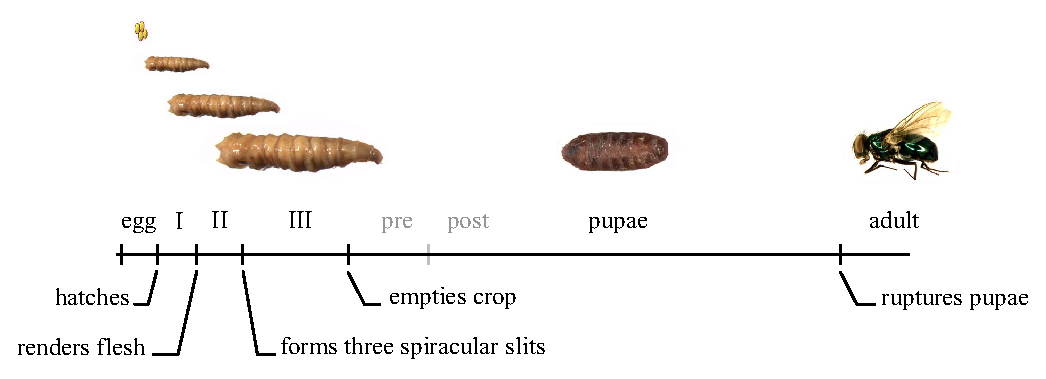
\includegraphics[width=\textwidth]{Figures/blowflycycle}
      \caption{Life cycle of blow fly showing relative time spent in
      each stage of development.}
  \end{figure}

\end{frame}

\subsection{Current methods}
\begin{frame}
Progression through an insect's life cycle is temperature dependent,
so thermal summation models are often used.
\begin{figure}
 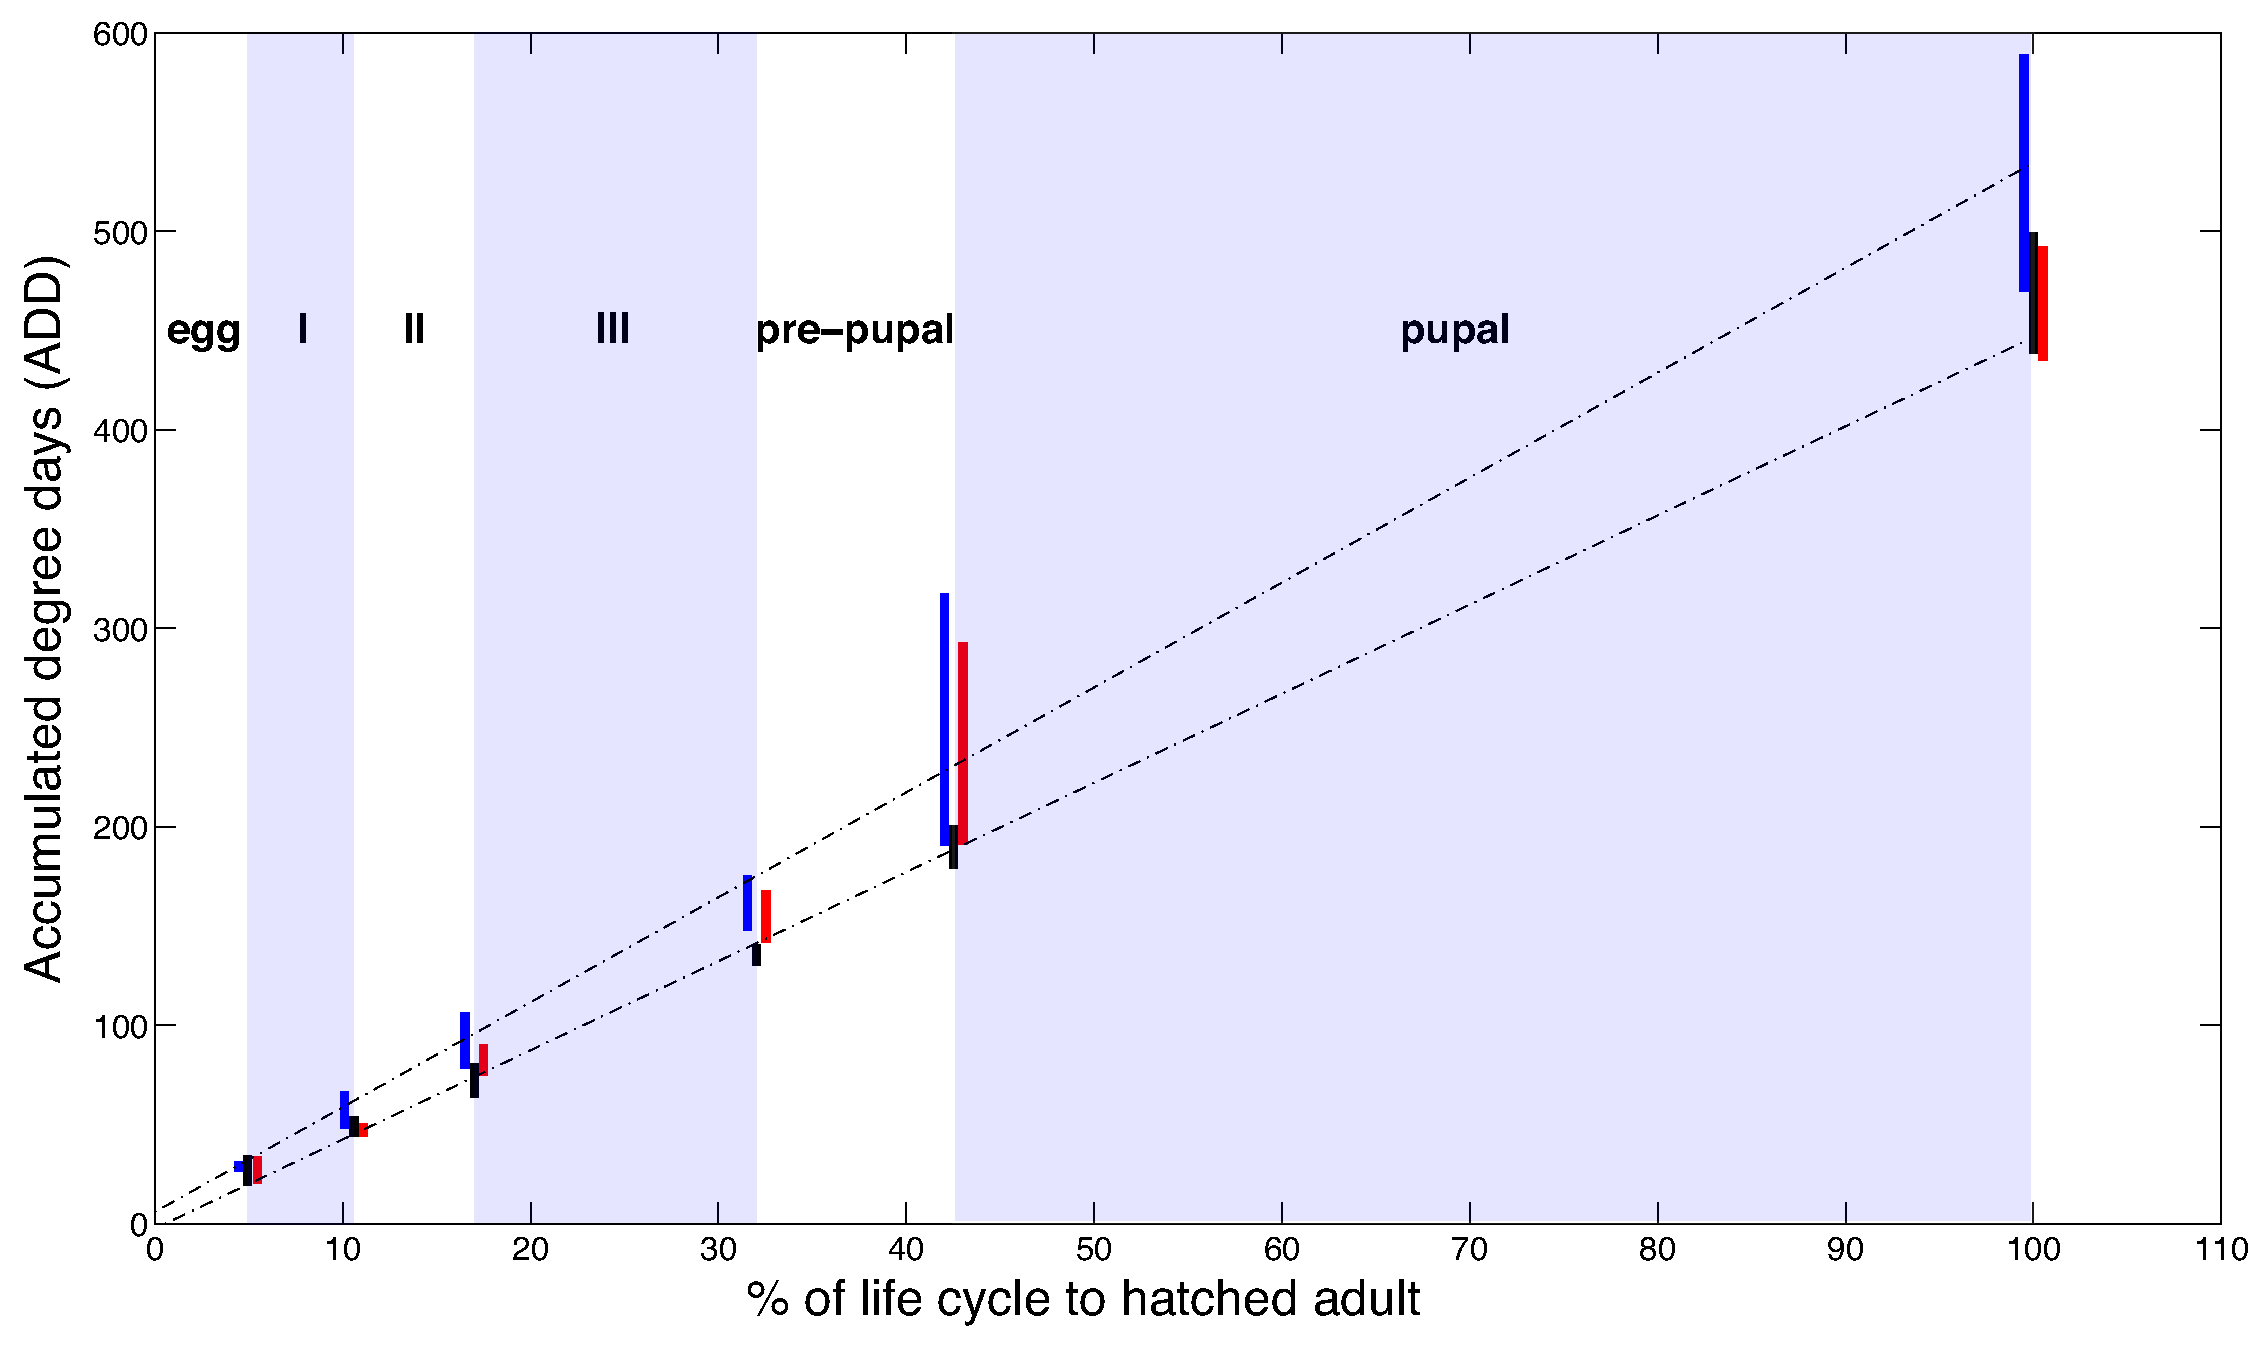
\includegraphics[width=0.8\textwidth]{Figures/anderson}
  \caption{Development data for Calliphoridae at three different temperature
profiles as collected in . The ADD range at
15.8~$^\circ$\textsf{C} (blue), 20.6~$^\circ$\textsf{C} (black), and 23.3~$^\circ$\textsf{C} (red)
are shown.  }
%\cite{Anderson2000}
\end{figure}
\end{frame}

\begin{frame}
  To use the thermal summation model historic temperature
  profiles are required. Current methods use linear regression between
  the environment and a simulated internal logger.
  \begin{figure}
    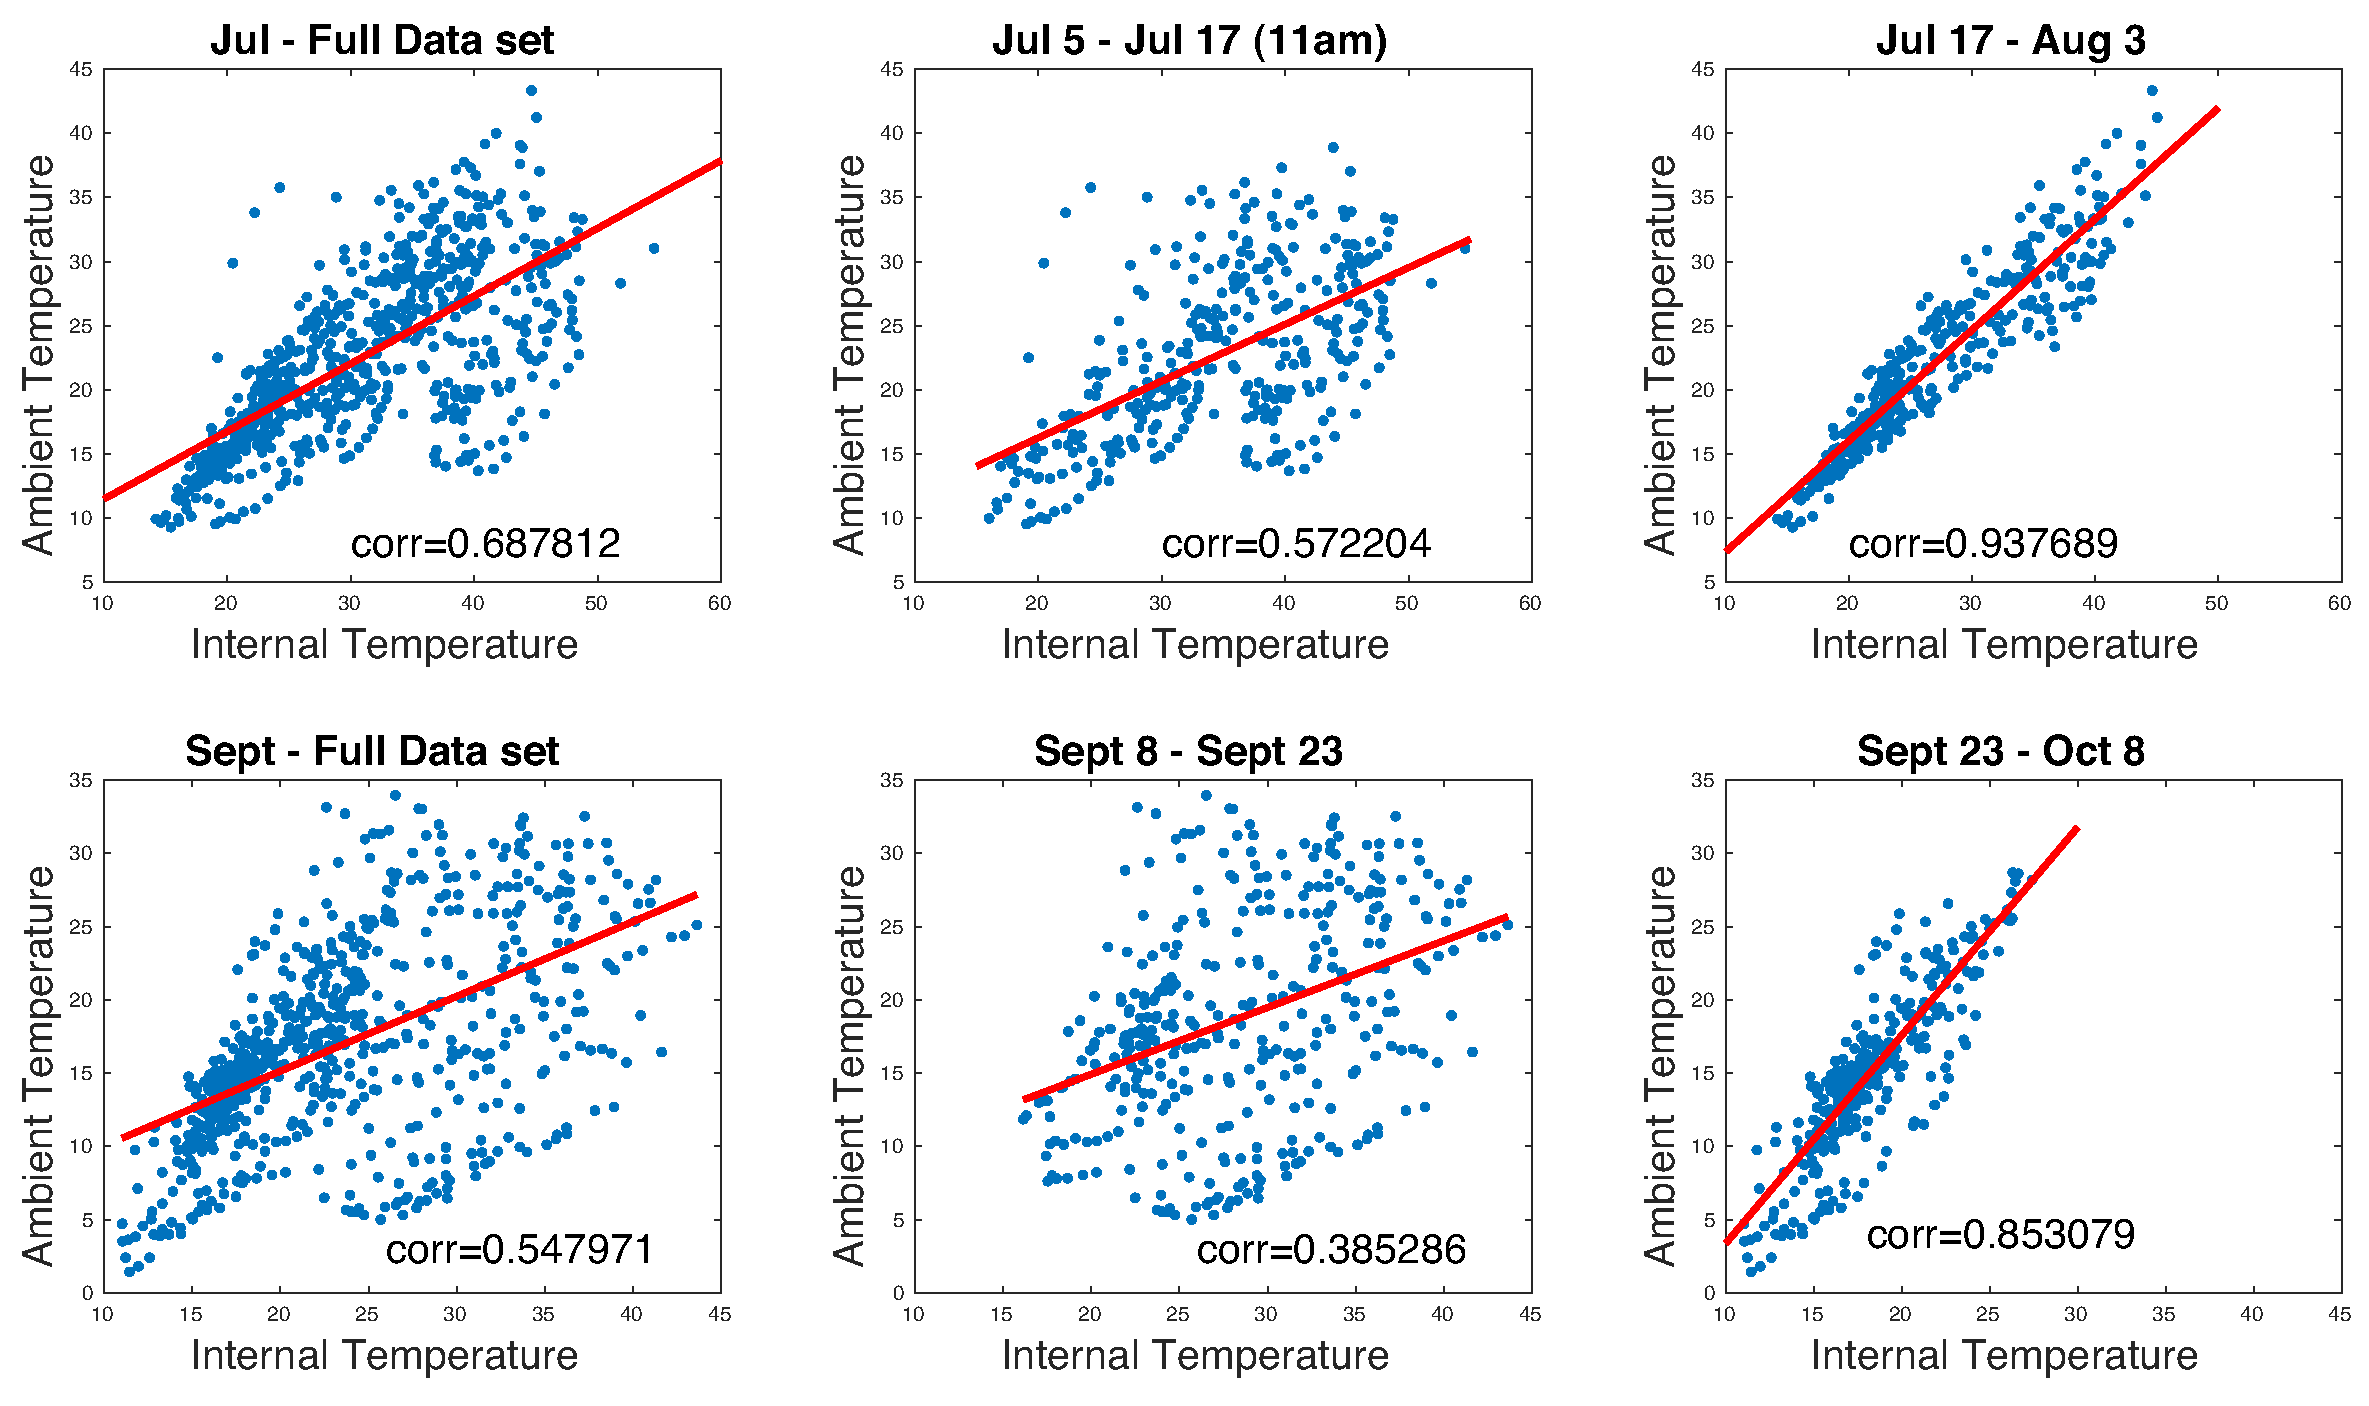
\includegraphics[width=0.9\textwidth]{Figures/correlation}
    \caption{Correlation figures for case study data from July and
      September 2016 decomposition studies performed with swine
      cadavers at Ontario Tech.}
  \end{figure}
\end{frame}

\section{Model Development}
\subsection{Motivation}
\begin{frame}
  Case study data offers internal logger measurements as well as
  ambient temperature measurement with nearby external loggers.
  \begin{figure}
    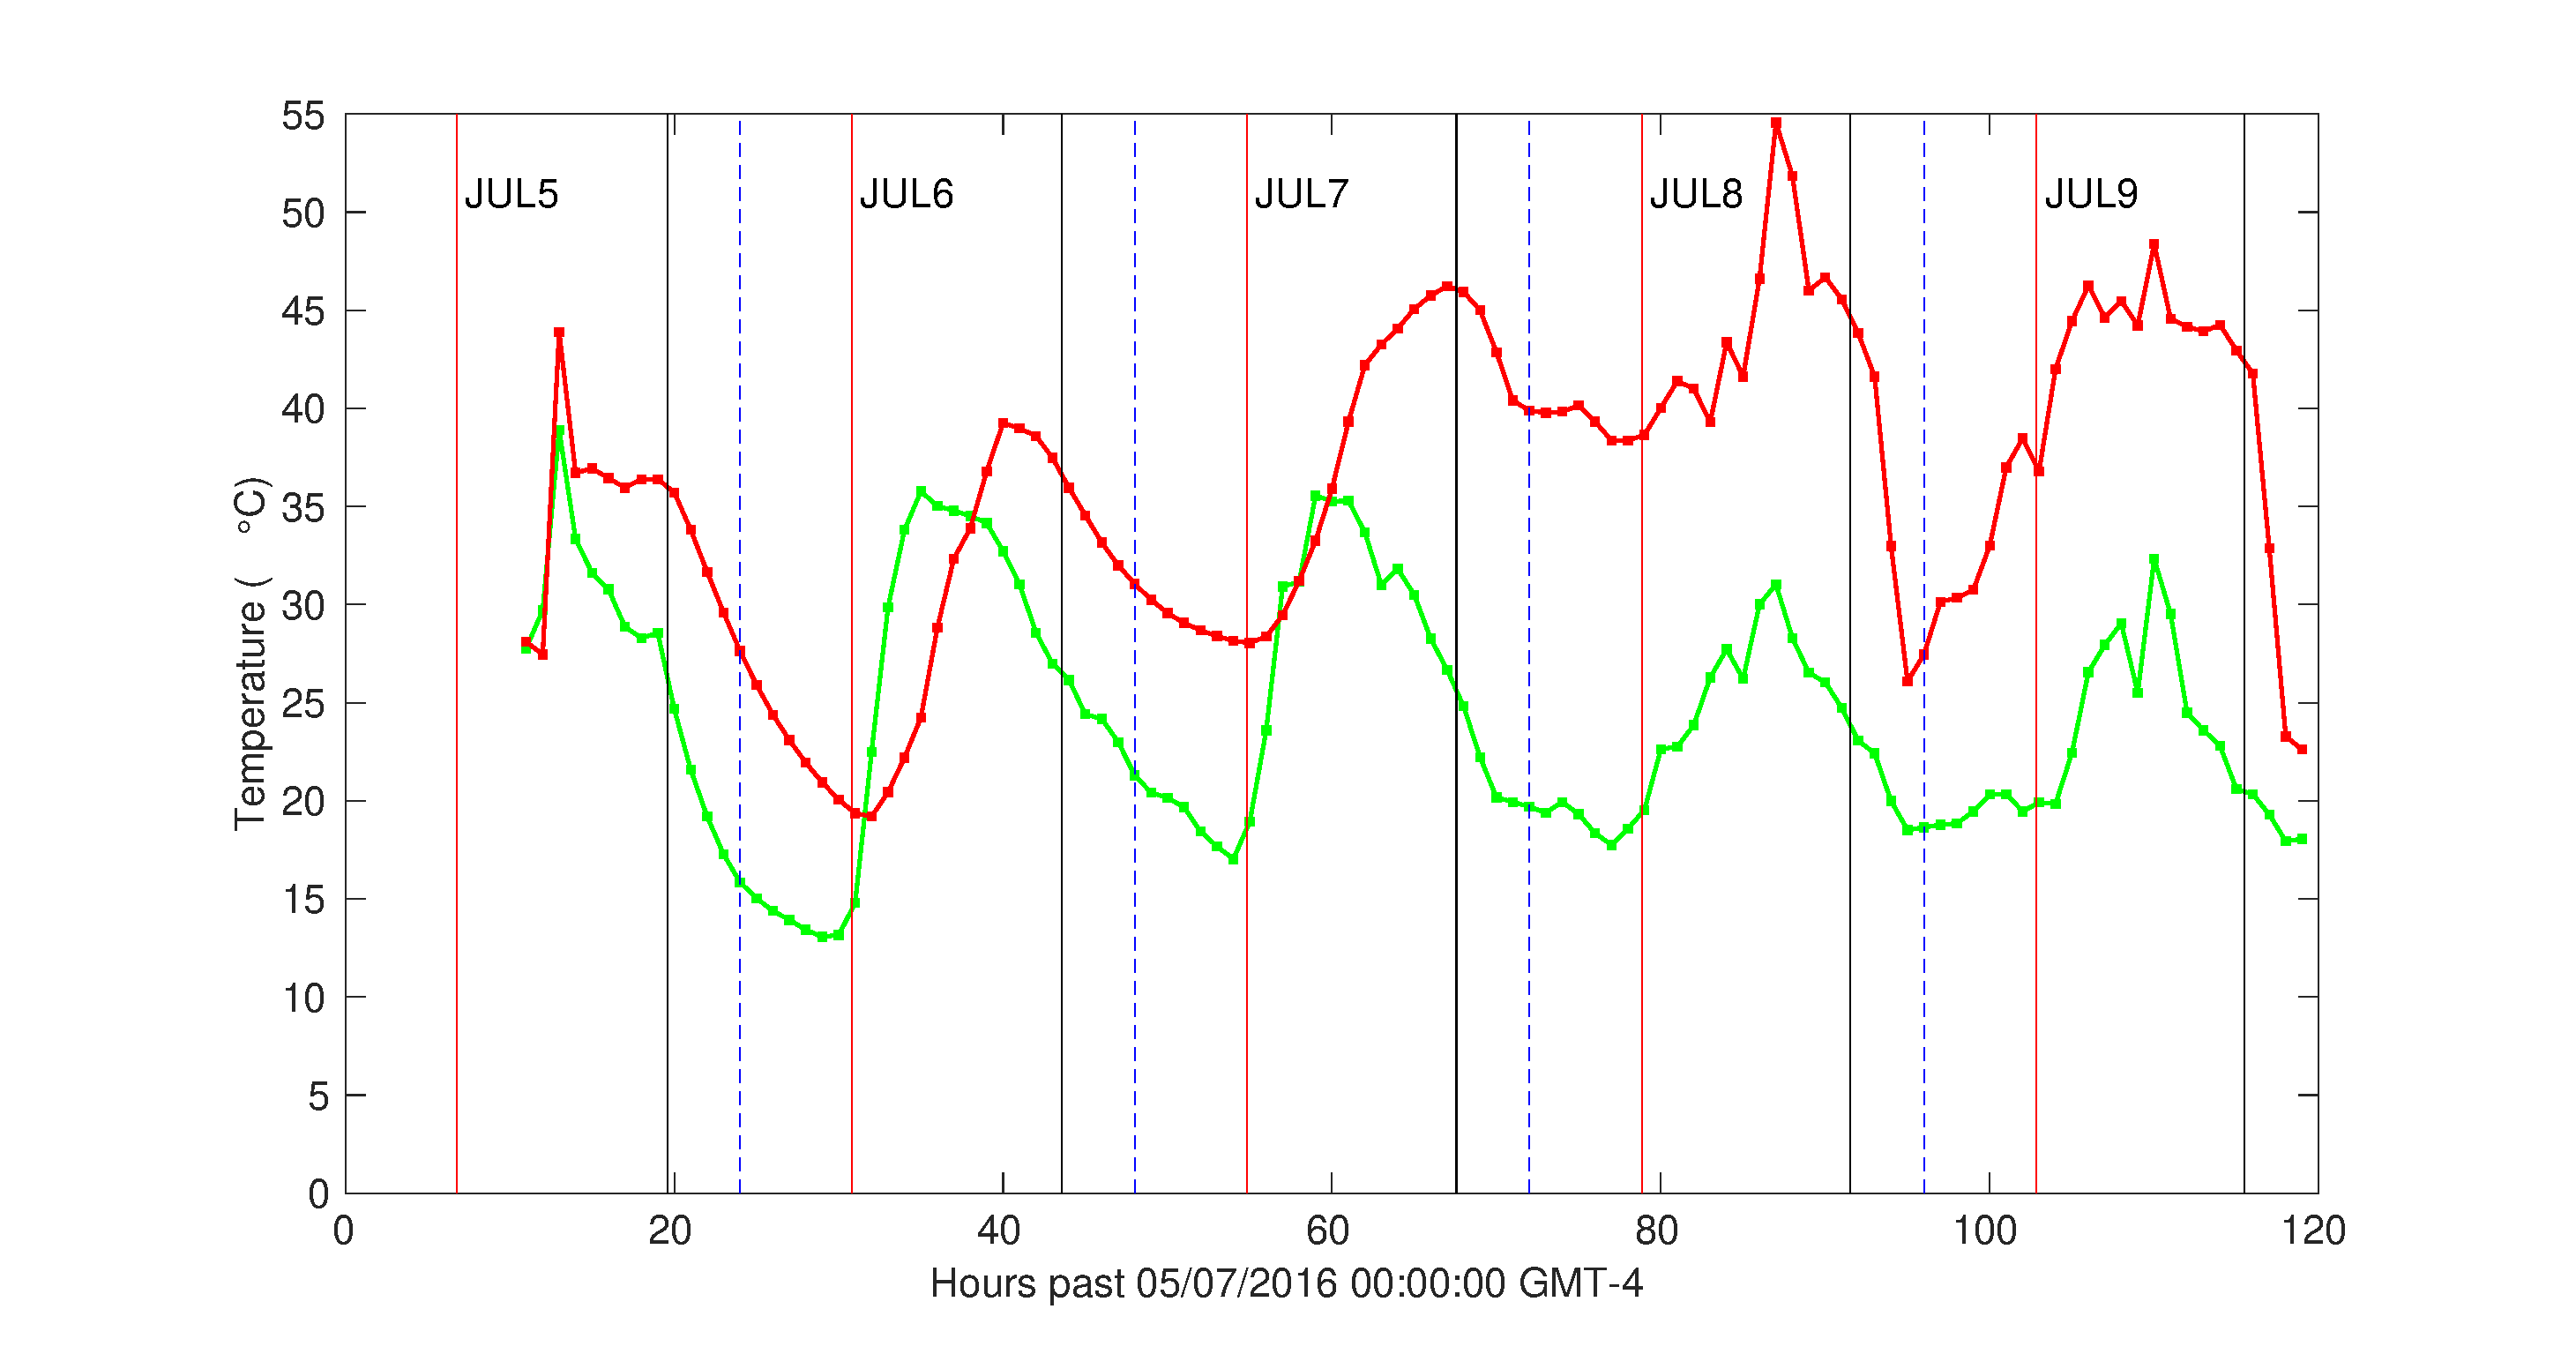
\includegraphics[width=0.9\textwidth]{Figures/jul1}
    \caption{Internal temperature probe (red) and environmental
      temperatures (green) for the first five days of a swine cadaver
      decomposition study in July 2016}

  \end{figure}

\end{frame}
\begin{frame}
  There are some notable patterns between the two temperature profiles
  \begin{itemize}
    \item There exists a phase shift between the two curves, especially
in the first few days;
\item The phase shift decreases over time;
\item The internal logger doesn't experience the same lows as
the ambient temperature, and experiences higher maximums;
\item Both temperature profiles have a distinct day/night cycle.

  \end{itemize}

\end{frame}
\subsection{Exploring a Toy model}
\begin{frame}
  We explore a heat equation approach. Starting with
  \begin{equation}\label{eq:heat}
\rho c_p \pd{T}{t} = k \nabla^2T + Q(\mathbf{x},t).
\end{equation}
We consider the model in cylindrical coordinates to
simulate a three dimensional cylindrical vessel, (\ref{eq:heat}) becomes
\begin{equation}
 \rho c_p \pd{T}{t} = k \left( \frac{\partial^2 T}{\partial^2 t} + 
    \frac{1}{r} \pd{T}{r} + \frac{\partial^2 T}{\partial^2 z}\right) + Q(r,z,t).
\end{equation}
\end{frame}

\begin{frame}
In terms of boundary conditions we desire that the vessel is insulated
on all sides and the bottom, $S_2, S_3$. The top, $S_1$, may interact
with the environment. This gives way to
\begin{align}
&-k \left.\pd{T}{\hat{n}}\right|_{S_2, S_3} = 0,  &-k \left.\pd{T}{\hat{n}}\right|_{S_1} = h(T - T_{\text{ext}}(t))
\end{align}
\end{frame}

\begin{frame}
  We examine the effects of averaging over the spacial dimensions to
  obtain an ordinary differential equation which is only time
  dependent. We rewrite the model where $\bar{\bar{T}}(t) \mapsto
  \bar{\theta}(\tau)$, 
  \begin{align}\label{eq:mod}
    \deriv{\bar{\theta}}{\tau} =-\frac{h\Delta T}{Q_0H}
    \left(\bar{\theta}-\theta_\text{ext}(\tau)\right)
    + q(\tau), 
    \quad\quad \bar{\theta}(0)=0.
  \end{align}
\end{frame}

\begin{frame}
  We run a simulation with a set of parameters to
  correspond to a bucket of water of depth 30~\textsf{cm} and a
  significant amount of internal heating. We allow external heating to
  be sinusoidal. We examine the solution to
  (\ref{eq:mod}) by solving the ODE numerically and with method of
  lines.
  \begin{figure}
    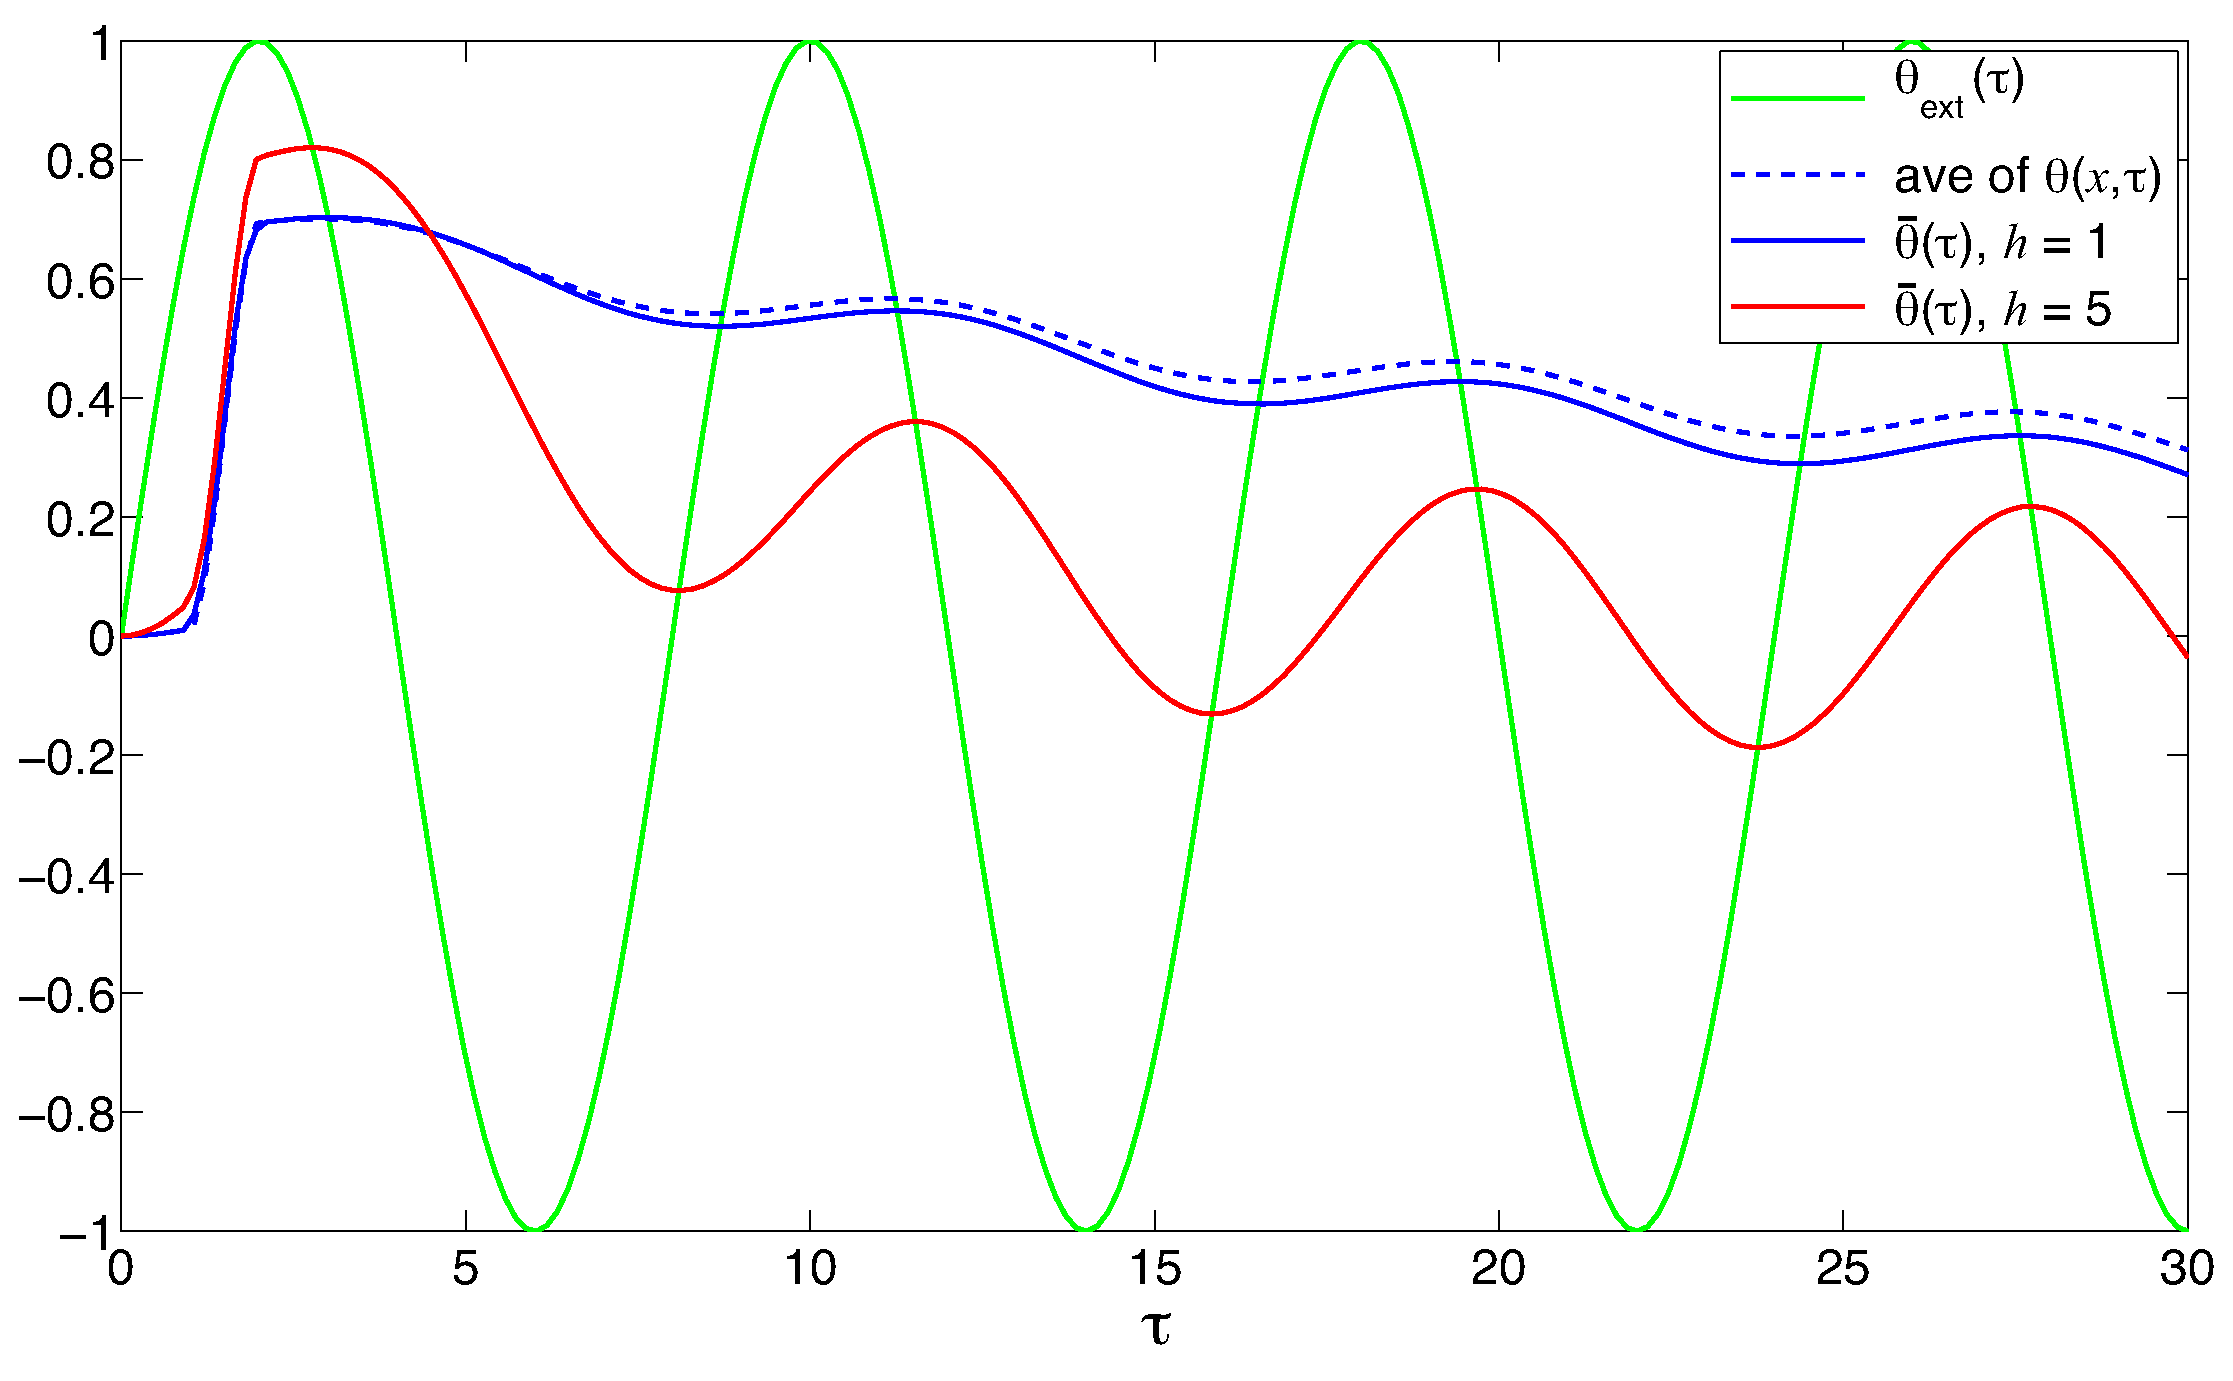
\includegraphics[width=0.7\textwidth]{Figures/toymodelcomp}
    \caption{Solution to the ODE with $h=1$ (blue), $h=5$ (red), using
    method of lines (dashed blue) and the external heating (green).}
  \end{figure}

\end{frame}

\subsection{Forward Problem}

\begin{frame}
  We use the toy model to inform the model for a swine cadaver. We
  allow for heat flux through the boundary,
  \begin{align}
\label{eq:model_bc}
    &- k \left.\pd{T}{\hat{n}}\right|_{\partial \Omega} = h(T-T_0)& 
    &\mathbf{x} \in \partial \Omega,\ t>0,
  \end{align}
  and simplify by averaging at every point so that the average
  temperature is
  \begin{equation}
\label{eq:avg}
    \bar{T}(t) = \frac{1}{|\Omega|}\int_{\Omega} 
    T(\mathbf{x}, t)\,\mathrm{d} \mathbf{x}.
  \end{equation}
  We nondimensionalize using
  \begin{align}
    &\bar{T} = T_{\text{min}} + \Delta T \theta&
    &T_0 = T_{\text{min}} + \Delta T\theta_0&
    &t = \tau \tilde{t}.
\end{align}
\end{frame}

\begin{frame}
 The equation for the averaged 
temperature, as derived analogous to the previous section, becomes
\begin{align}
\label{eq:aveode}
    \deriv{\theta}{t} = 
    c(t)(\theta_0(t) - \theta) + s(t),
\end{align}
with
\begin{align}
\label{params}
    c(t) &= \frac{h|\partial \Omega|\tau}{\rho c_p|\Omega|},&
    s(t) &= \frac{Q(t)\tau}{\rho c_p\Delta T},&
    Q(t) &= \frac{1}{|\Omega|}\int_{\Omega}
    q(\mathbf{x},t)\,\mathrm{d} \mathbf{x},
\end{align}
\end{frame}

\section{Parameter Investigation}
\begin{frame}
  We choose the coupling coefficient to be a constant, $c(t) \mapsto
  c_0$ and the heat flux, $s(t)$, to be piecewise constant with
  changes at characteristic times, $\tau_j$, corresponding to sunrise
  and sunset.
  \begin{figure}[t]
    \centering
% Drawing of the time intervals with c(t) and s(t) dependence
\setlength{\unitlength}{1cm}
\begin{picture}(10,2.3)
\put(0,1){[\hspace{5mm}$I_0$\hspace{5mm})}
\put(1.6,1){[\hspace{5mm}$I_1$\hspace{5mm})}
\put(4.1,1){$\ldots$}
\put(5.5,1){[\hspace{5mm}$I_N$\hspace{5mm})}
%\put(8,1){$\ldots$}
%\put(9.5,1){[\hspace{5mm}$I_N$\hspace{5mm})}
\put(-1,1.7){$s(t)$:}
\put(0.7,1.7){$s_0$}
\put(2.3,1.7){$s_1$}
\put(6.2,1.7){$s_N$}
%\put(10.2,1.7){$s_N$}
\put(-1,2.3){$c(t)$:}
\put(0.7,2.3){$c_0$}
\put(2.3,2.3){$c_0$}
\put(6.2,2.3){$c_0$}
%\put(10,2.3){$c_0$}
\thicklines
% Draw the axis
\put(-1,0.7){\vector(1,0){10}}
% Tickmarks
\put(0.08,0.6){\line(0,1){0.2}}
\put(1.7,0.6){\line(0,1){0.2}}
\put(3.3,0.6){\line(0,1){0.2}}
\put(5.57,0.6){\line(0,1){0.2}}
\put(7.1,0.6){\line(0,1){0.2}}
%\put(9.57,0.6){\line(0,1){0.2}}
%\put(11.3,0.6){\line(0,1){0.2}}
% Extended dashed lines to bind the 
% c/s to the number line
{\color{gray}
\multiput(0.08,1.5)(0,0.2){7}{\line(0,1){0.1}}
\multiput(1.7,1.5)(0,0.2){7}{\line(0,1){0.1}}
\multiput(3.3,1.5)(0,0.2){7}{\line(0,1){0.1}}
\multiput(5.57,1.5)(0,0.2){7}{\line(0,1){0.1}}
\multiput(7.1,1.5)(0,0.2){7}{\line(0,1){0.1}}
%\multiput(9.57,1.5)(0,0.2){7}{\line(0,1){0.1}}
%\multiput(11.3,1.5)(0,0.2){7}{\line(0,1){0.1}}
}
% Labels
\put(0,0.3){$\tau_0$}
\put(1.6,0.3){$\tau_1$}
\put(3.2,0.3){$\tau_2$}
\put(5.5,0.3){$\tau_N$}
\put(7.0,0.3){$\tau_{N+1}$}
%\put(9.5,0.3){$\tau_N$}
%\put(11.2,0.3){$\tau_{N+1}$}
% Location of t
\put(6.25,0.3){$t$}
\end{picture}
\caption{The structure of $c(t)$ and $s(t)$.}
    \label{fig:c_and_s_structure}
\end{figure}
\end{frame}

\begin{frame}
  Upon rewriting the solution of (\ref{eq:aveode}) as $\theta = u +
  v$, to represent two heat sources we obtain a solution in the
  following form
  \begin{align}
\label{mywholemodel}
    \theta(t;c_0,\mathbf{s}) &= \theta(t_0)
    \textrm{e}^{-c_0(t-\tau_0)} + 
    c_0\int_{\tau_0}^t \textrm{e}^{-c_0(t-\eta)} 
    \theta_0(\eta)\, \diff \eta \\
    & \quad 
    + \frac{1}{c_0}\sum_{j=0}^{l-1}s_j
    \left(\textrm{e}^{-c_0(t-\tau_{j+1})}
    -\textrm{e}^{-c_0(t-\tau_j)}\right)
    + \frac{s_l}{c_0} \left(
    1-\textrm{e}^{-c_0(t-\tau_l)}\right),
\end{align}
for $\tau_l\le t<\tau_{l+1}$, and $l = 0, 1, \ldots, N$.
\end{frame}

\begin{frame}
With the model representation now having one values for $c_0$ and
$N+1$ values for $s$, we are able to use ground truth values to
perform a one parameter optimization. Ground truth measured internal temperatures, $\hat{\theta}$ are used to
give the objective function 
\begin{align}
\label{eq:min-f}
    f = \|\hat{\theta} - \theta\|^2_{\ell^2(\mathbb{R}^M)}.
\end{align}
\end{frame}

\begin{frame}

Or using a matrix approach 
\begin{align}
\label{eq:thetavec}
    \theta = \mathbf{u}(c_0) + B(c_0) \mathbf{s}
\end{align}
 where $\mathbf{u}(c_0) = (u(t_1;c_0),\ldots,u(t_M;c_0))^{\textsf{T}}$, and
 \begin{align}
 \label{bdefn}
     [B(c_0)]_{ij} = \frac{1}{c_0}\begin{cases}
     \textrm{e}^{-c_0(t_i-\tau_j)}-\textrm{e}^{-c_0(t_i-\tau_{j-1})}, &
     1 \le j \le l,\\
     1-\textrm{e}^{-c_0(t_i-\tau_l)}, & j = l+1,\\
     0, & l+2 \le j \le N+1.
     \end{cases}
 \end{align} 
\end{frame}

\section{Optimal Parameters}
\subsection{Coupling Coefficient}
\begin{frame}
Analysis of the coupling coefficient is performed by examining the
percent relative error
\begin{align}
\label{myrelerror}
    \textrm{Percent relative error} = 
    \frac{100}{\|\hat{\theta}\|_{\ell^2(\mathbb{R}^M)}}
    \left\|\left(\mathbf{I}- B(B^{\textsf{T}}B)^{-1}B^{\textsf{T}}\right)
    (\mathbf{u}-\hat{\theta})\right\|_{\ell^2(\mathbb{R}^M)}.
\end{align}

\begin{figure}
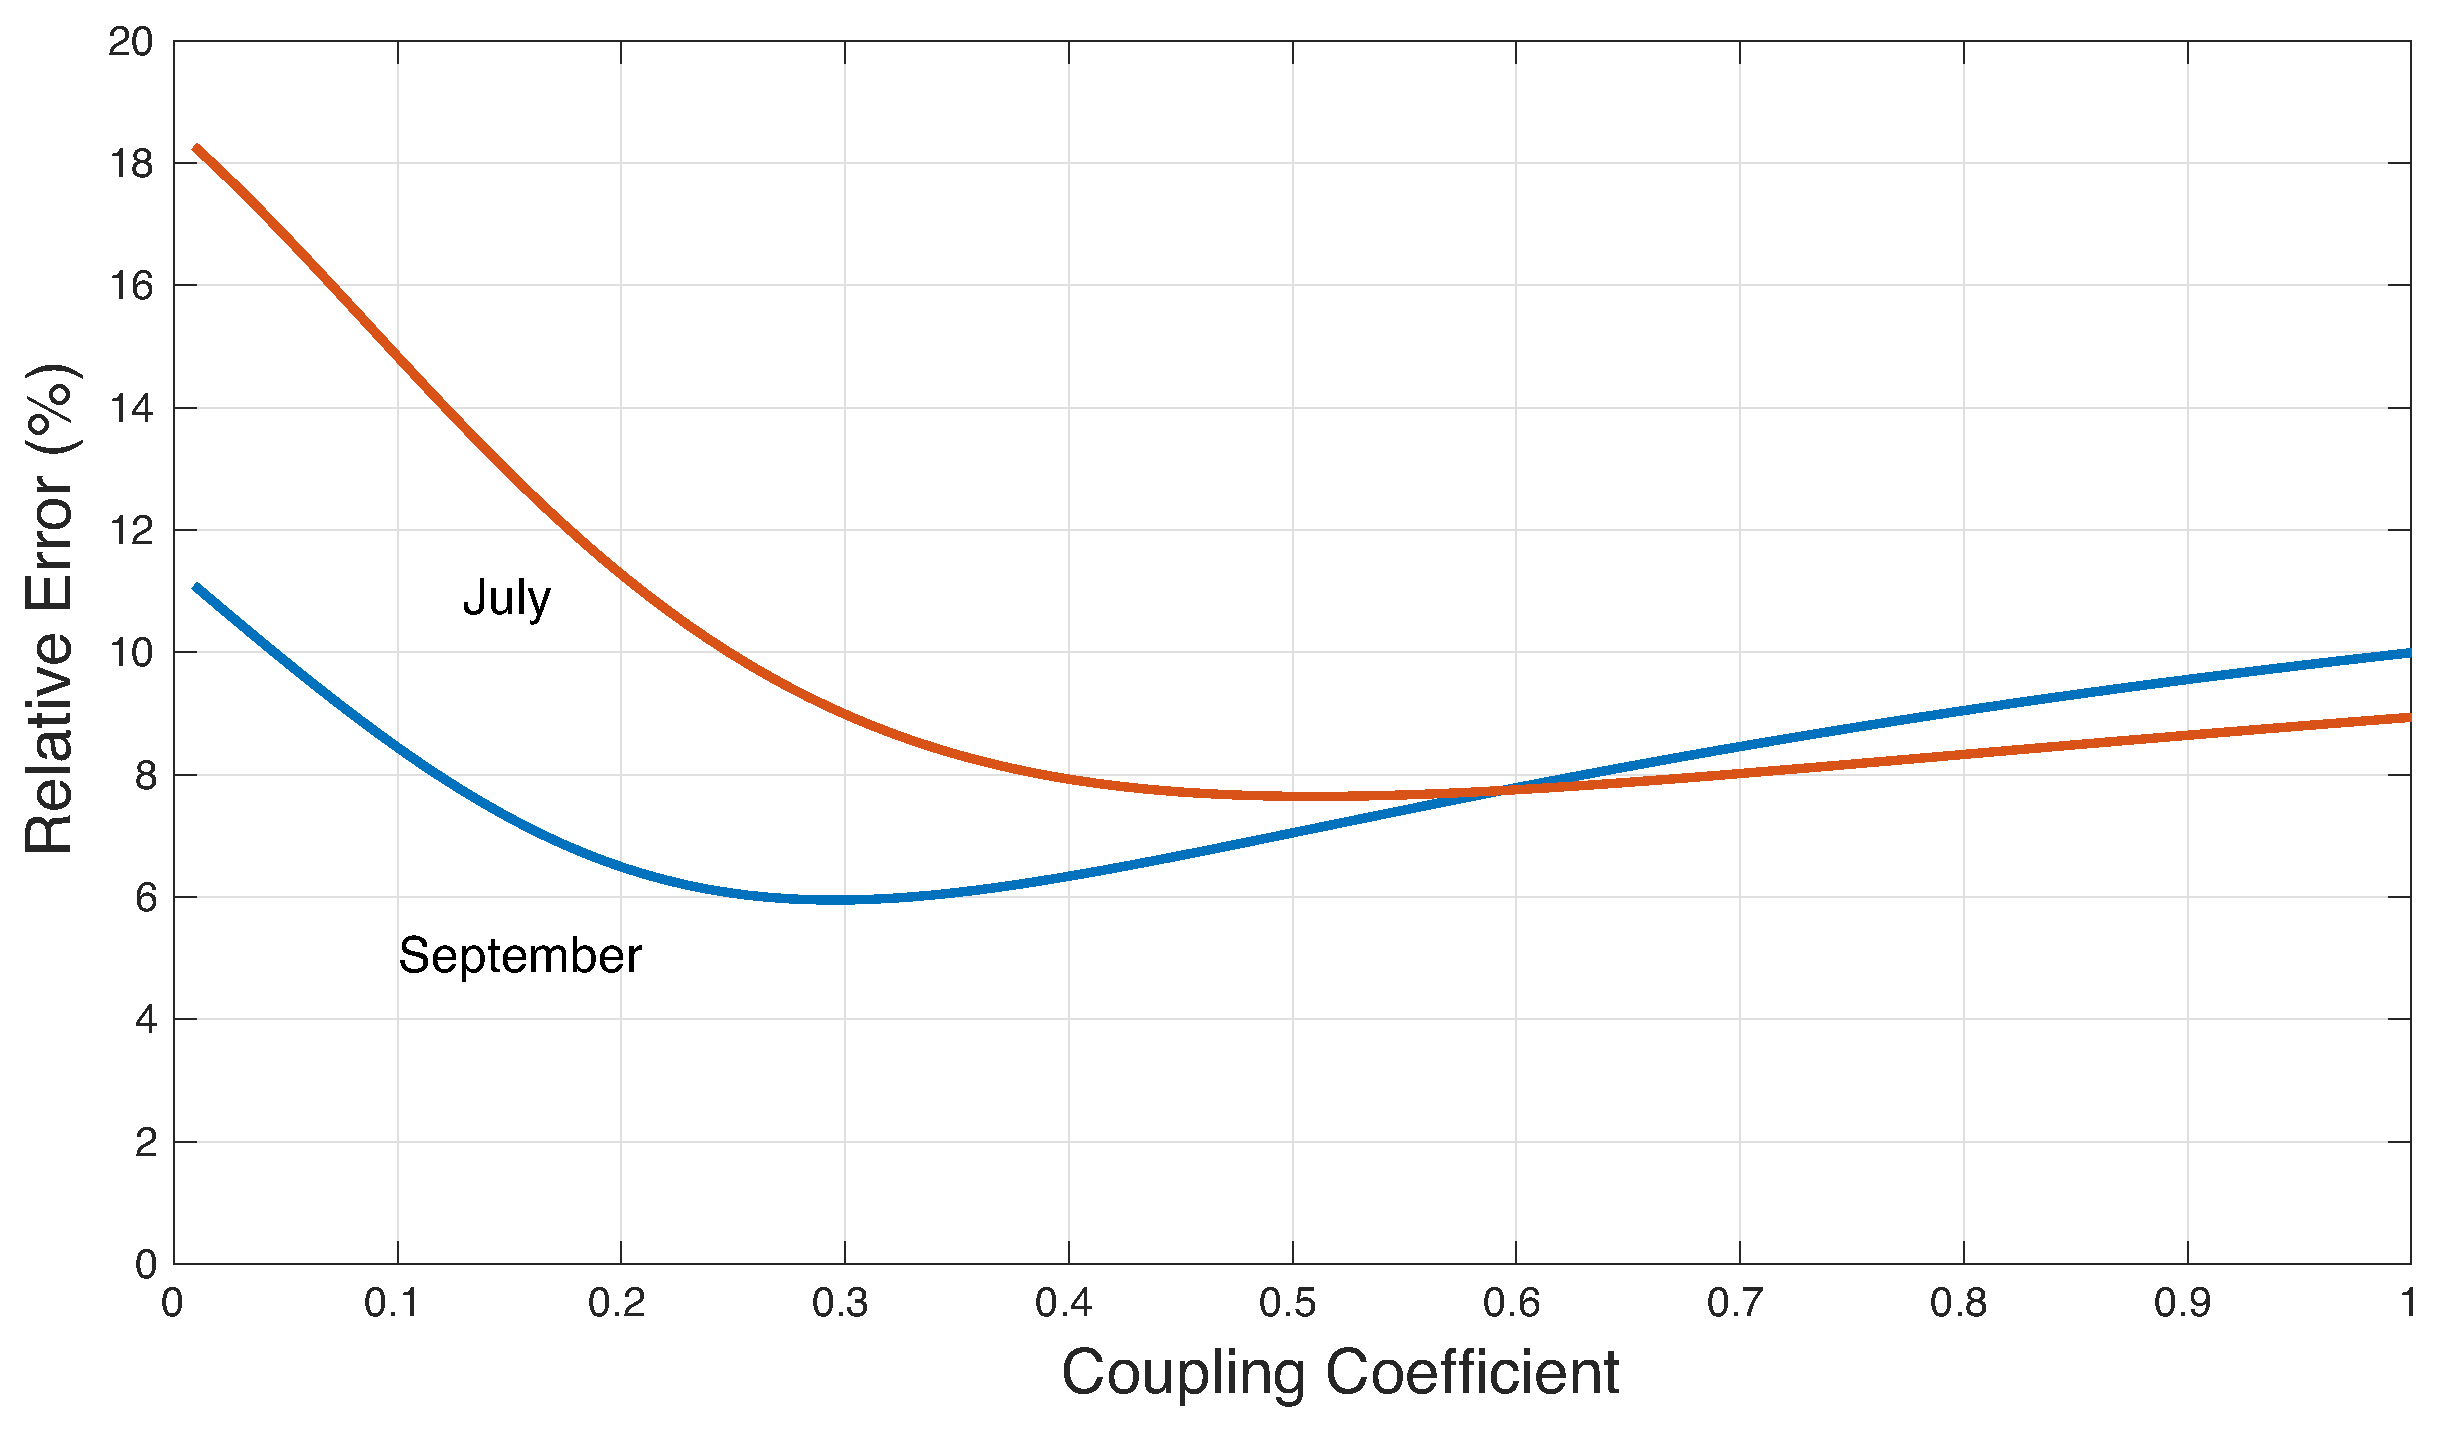
\includegraphics[width=0.8\textwidth]{Figures/sept_jul_err_n}
\end{figure}
\end{frame}

\begin{frame}
We also examine how the error and values of the coupling coefficient
changes as a function of time.
\begin{figure}
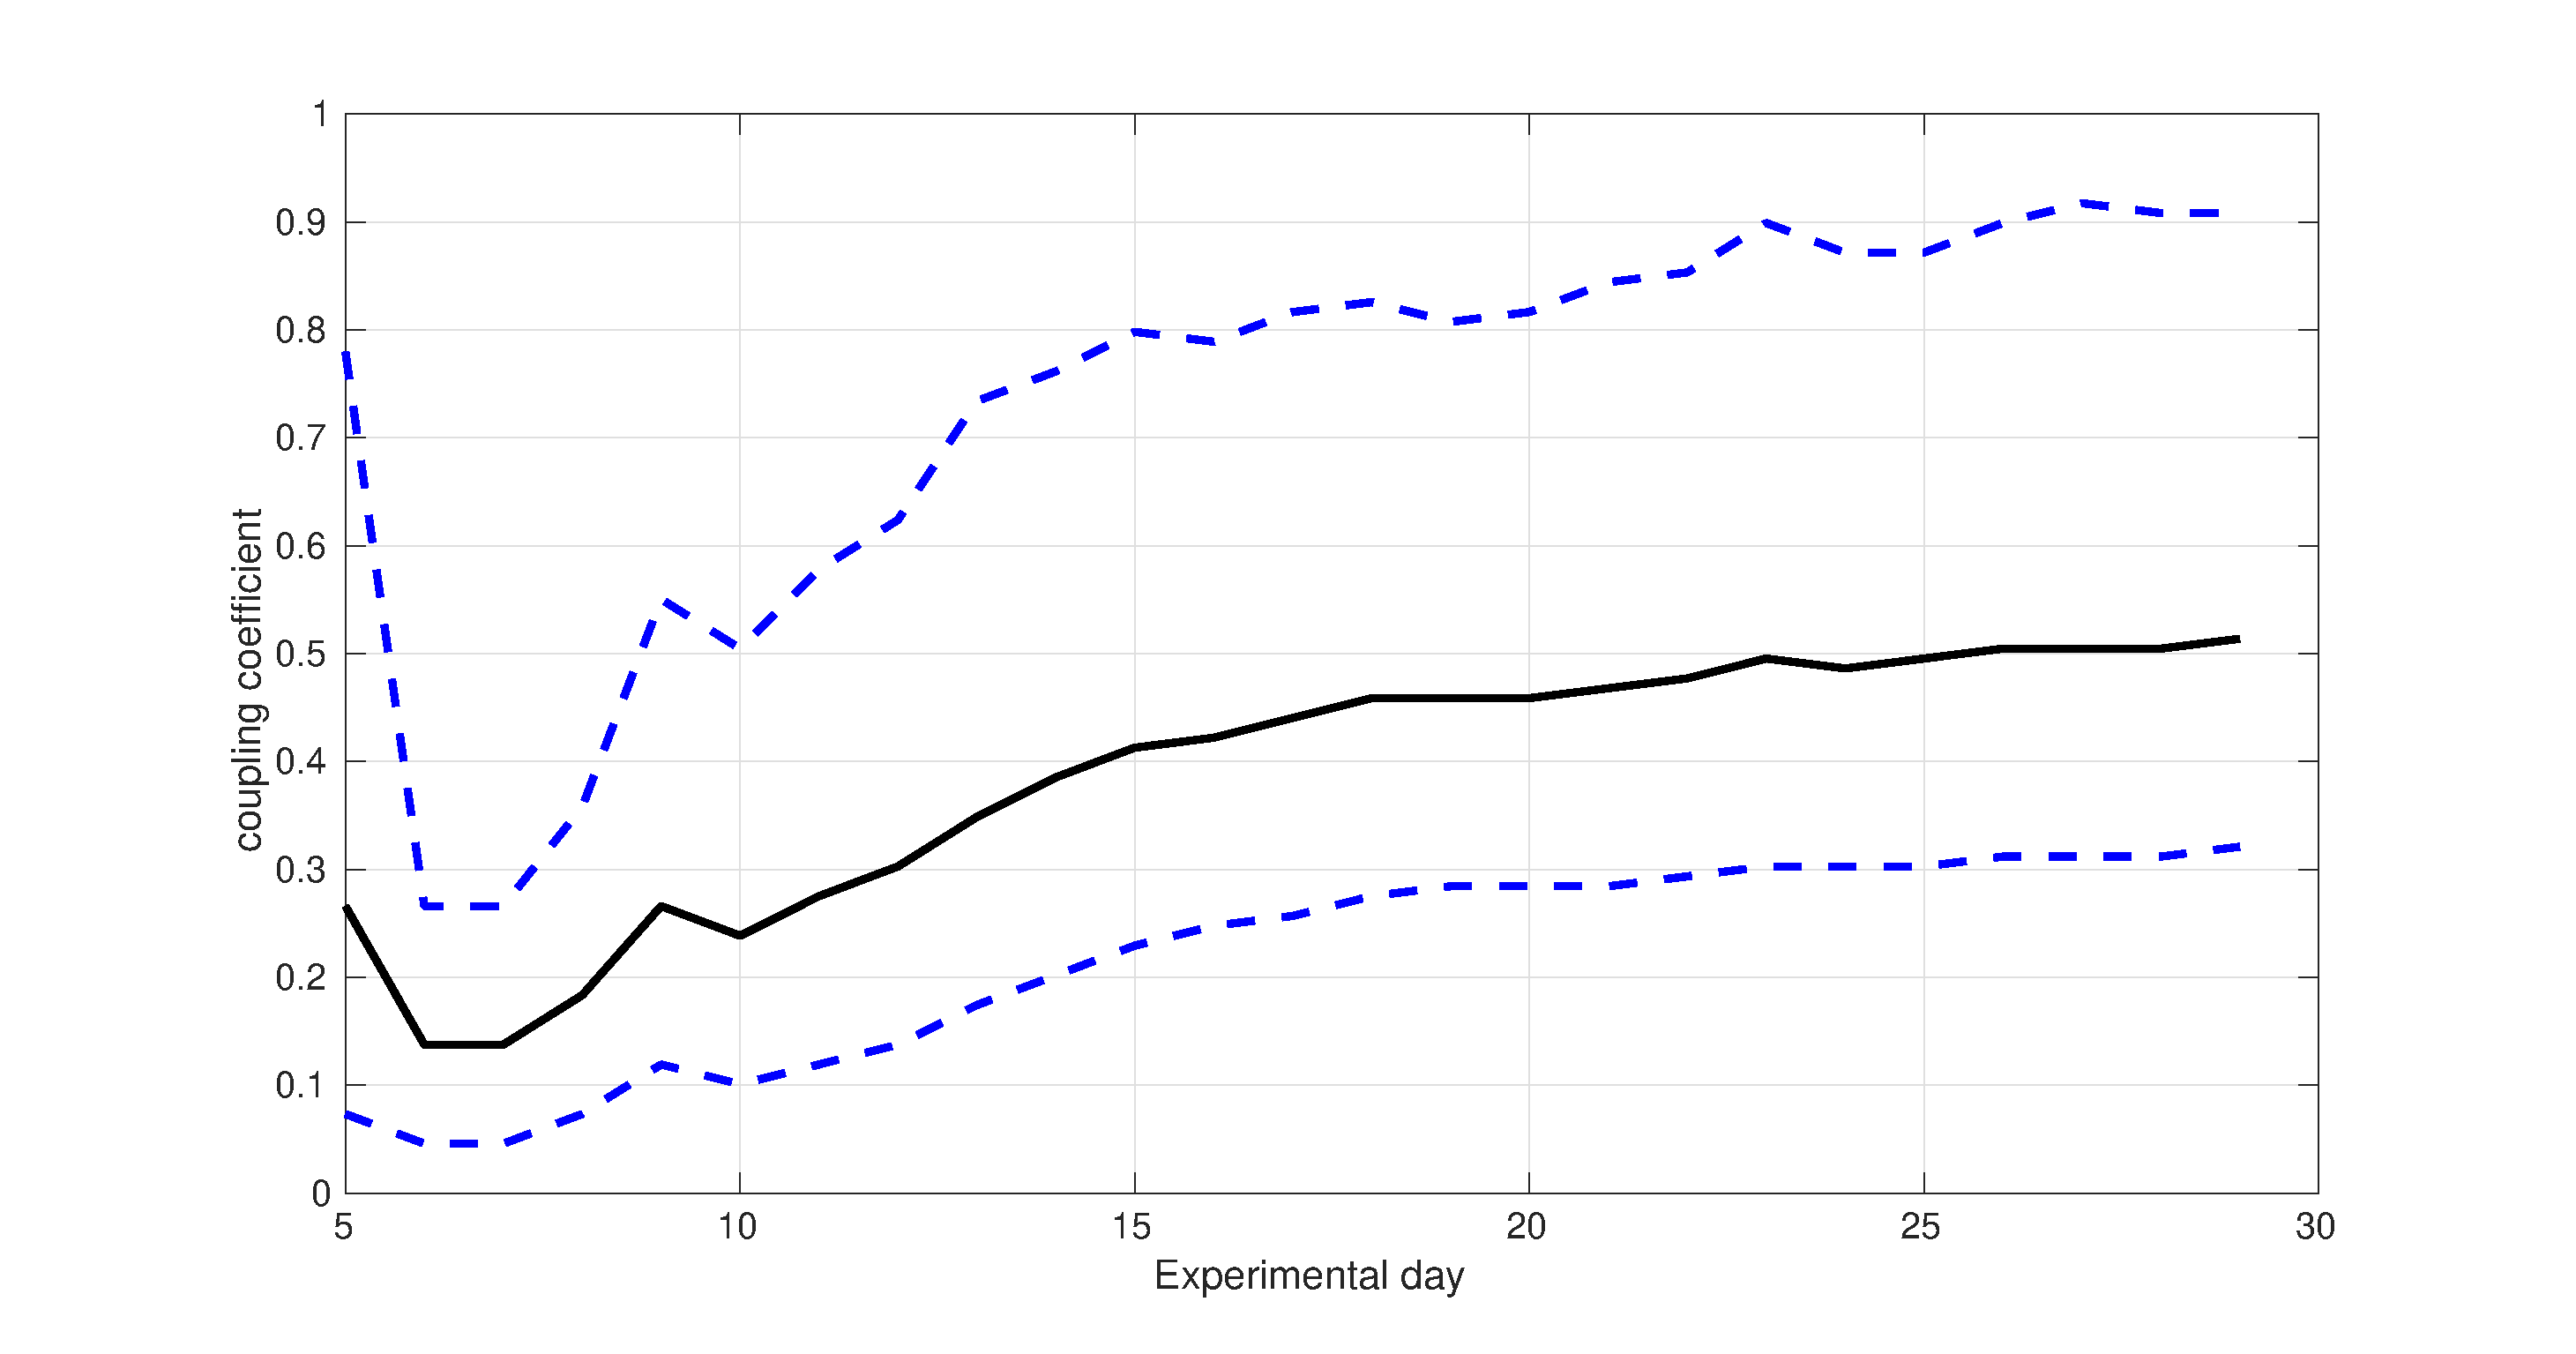
\includegraphics[width=0.49\textwidth]{Figures/jul_c_bounds}
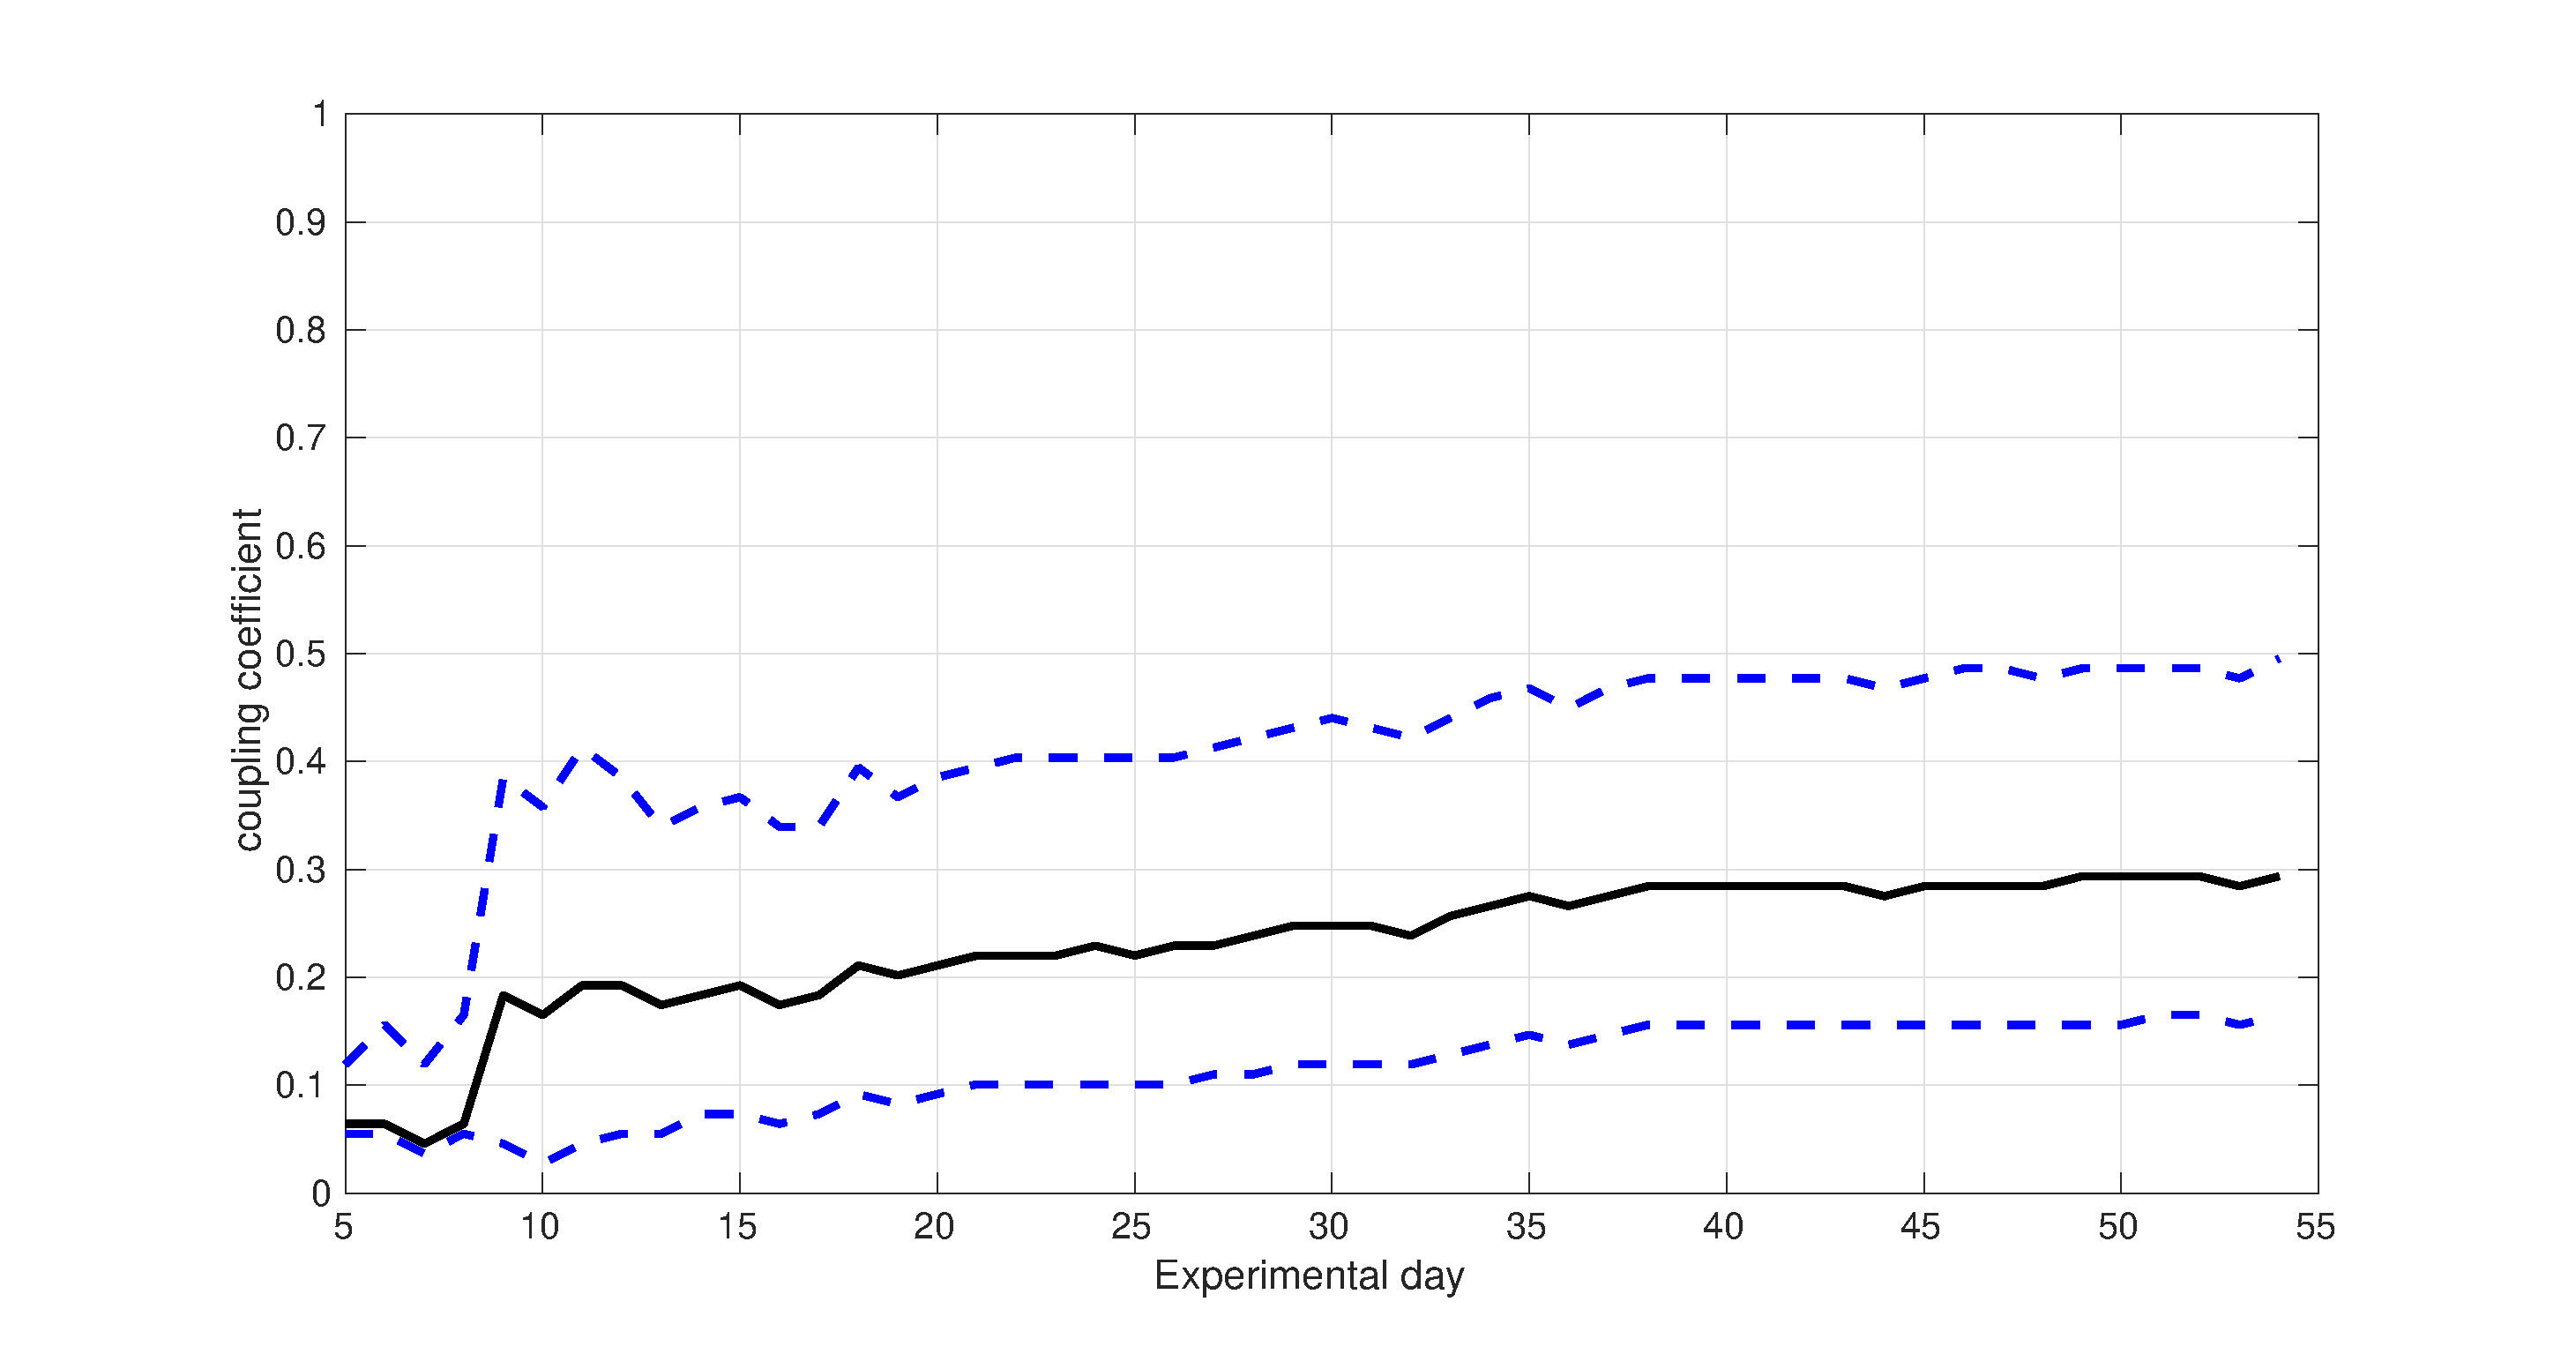
\includegraphics[width=0.49\textwidth]{Figures/sept_c_bounds2}
\caption{Left: July data set. Right:September data set. Upper and
  lower 1\% errors shown in dashed blue.}
\end{figure}

\end{frame}

\subsection{Heat Flux}
\begin{frame}
After finding the optimal choice of coupling coefficient we are able
to extract the optimal piecewise constant heat flux signature.
\begin{figure}
  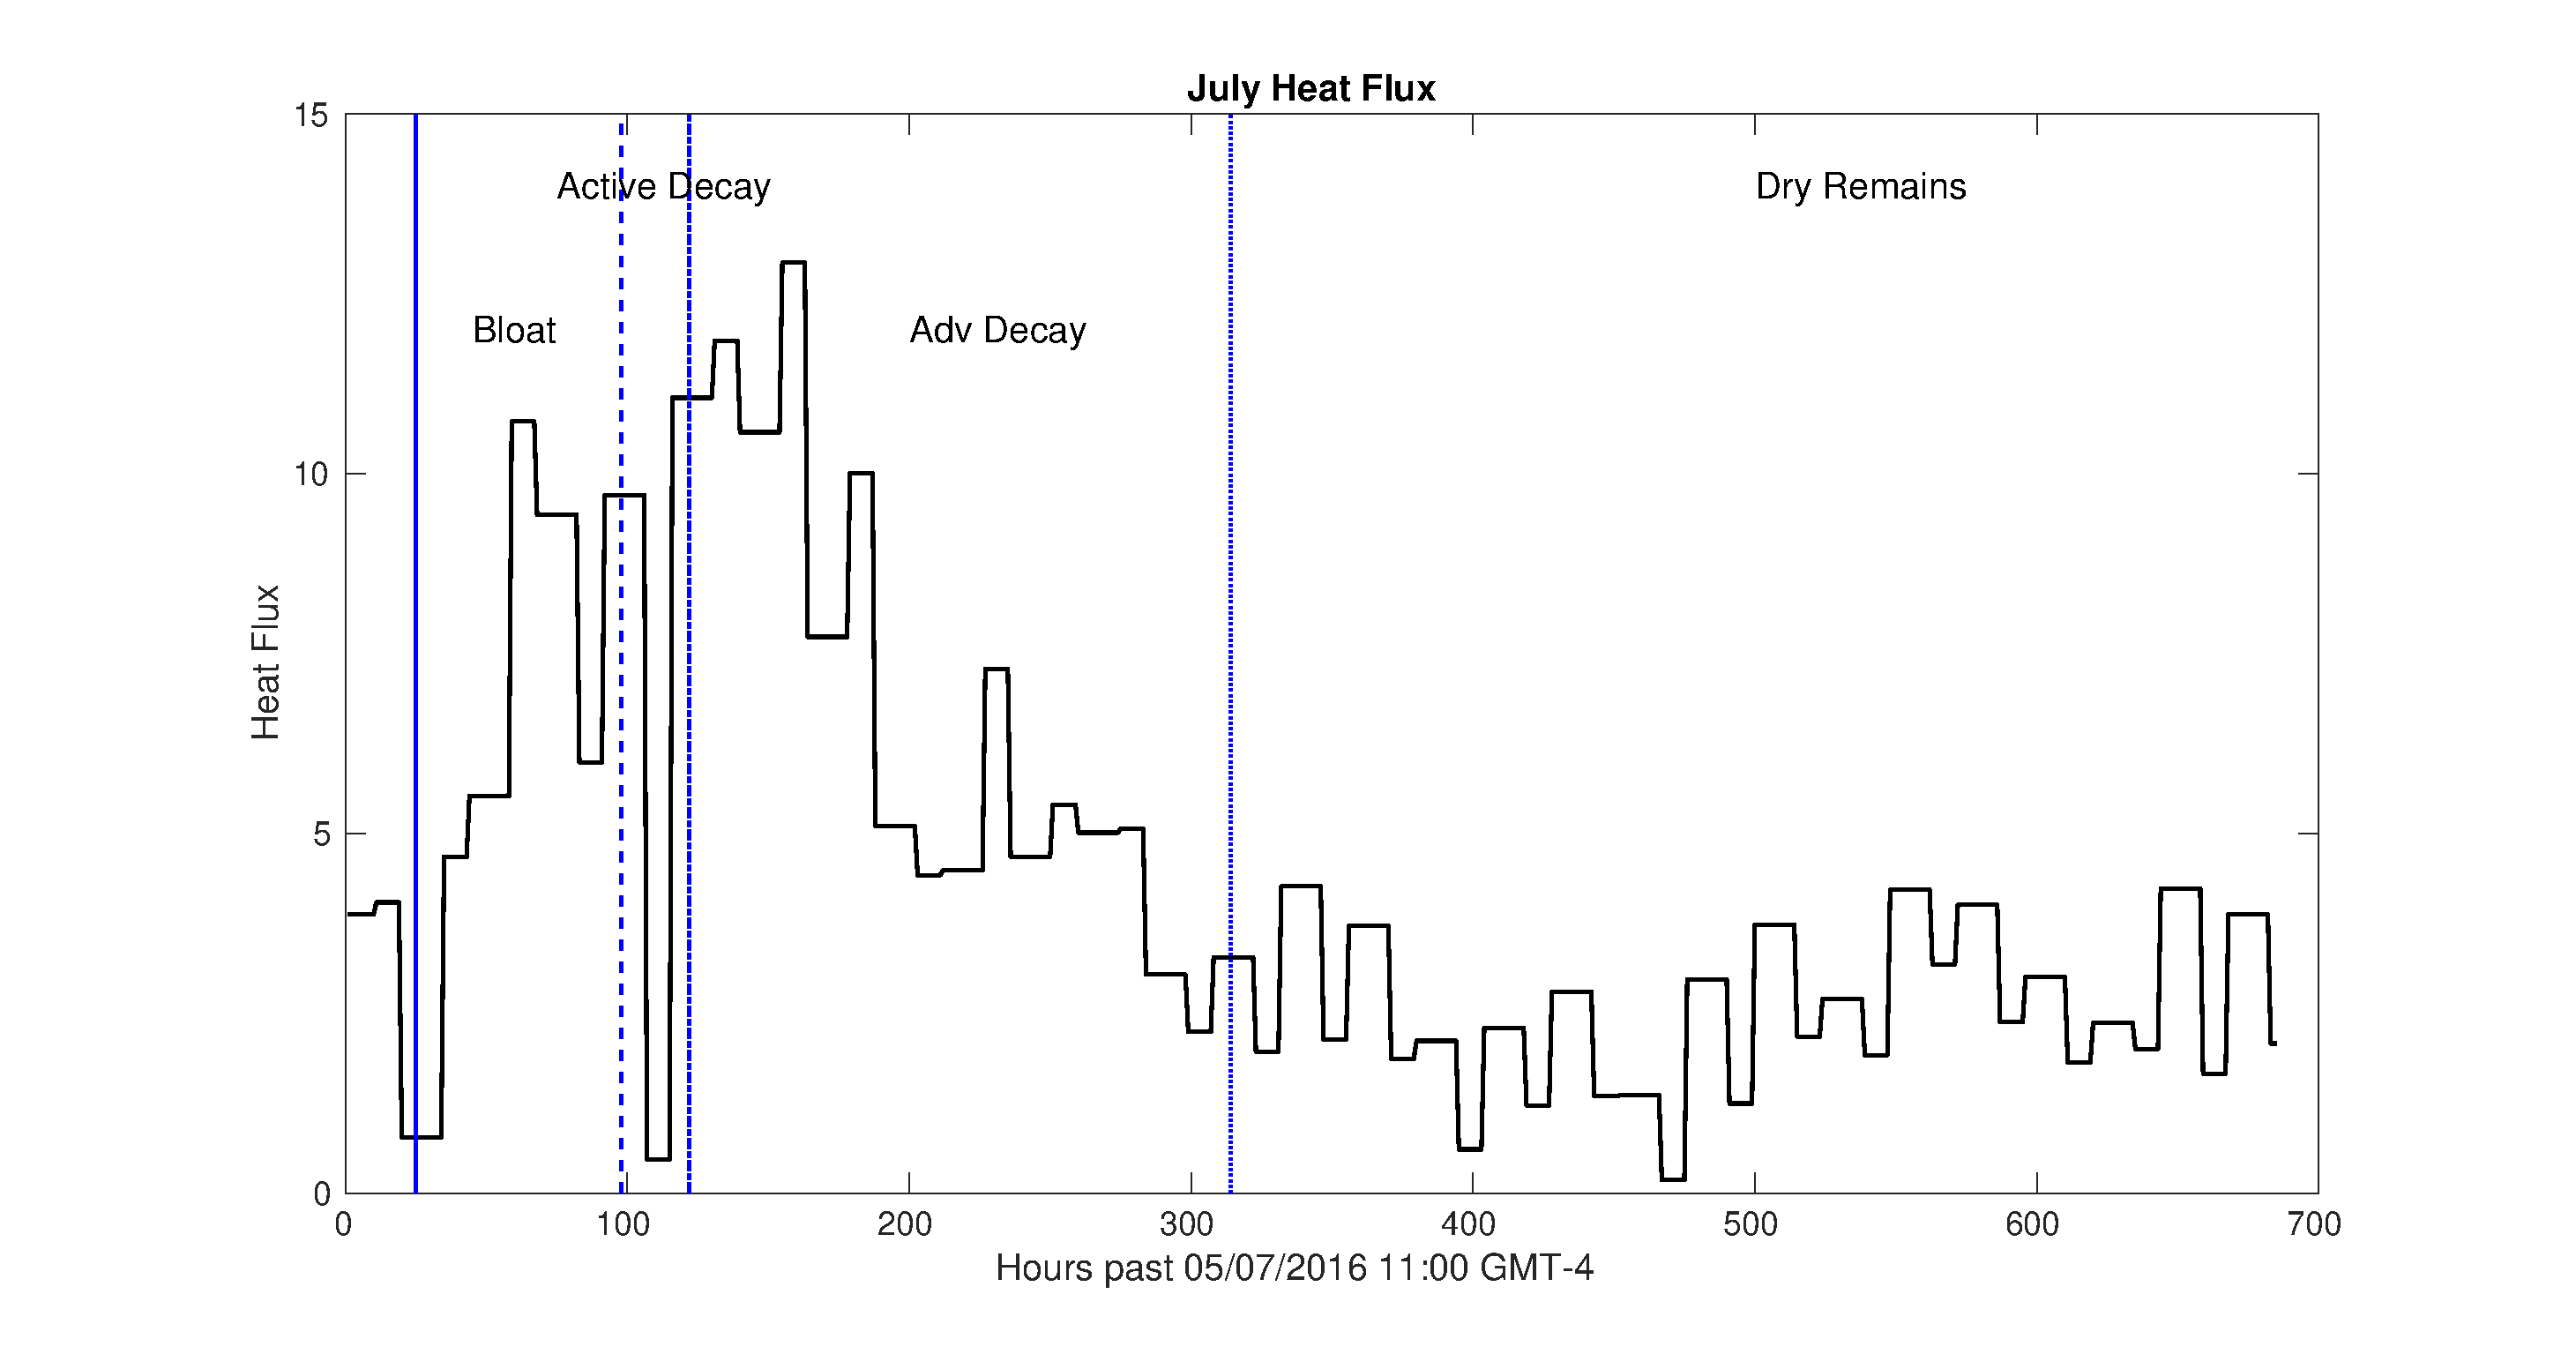
\includegraphics[width=0.49\textwidth]{Figures/jul_s}
  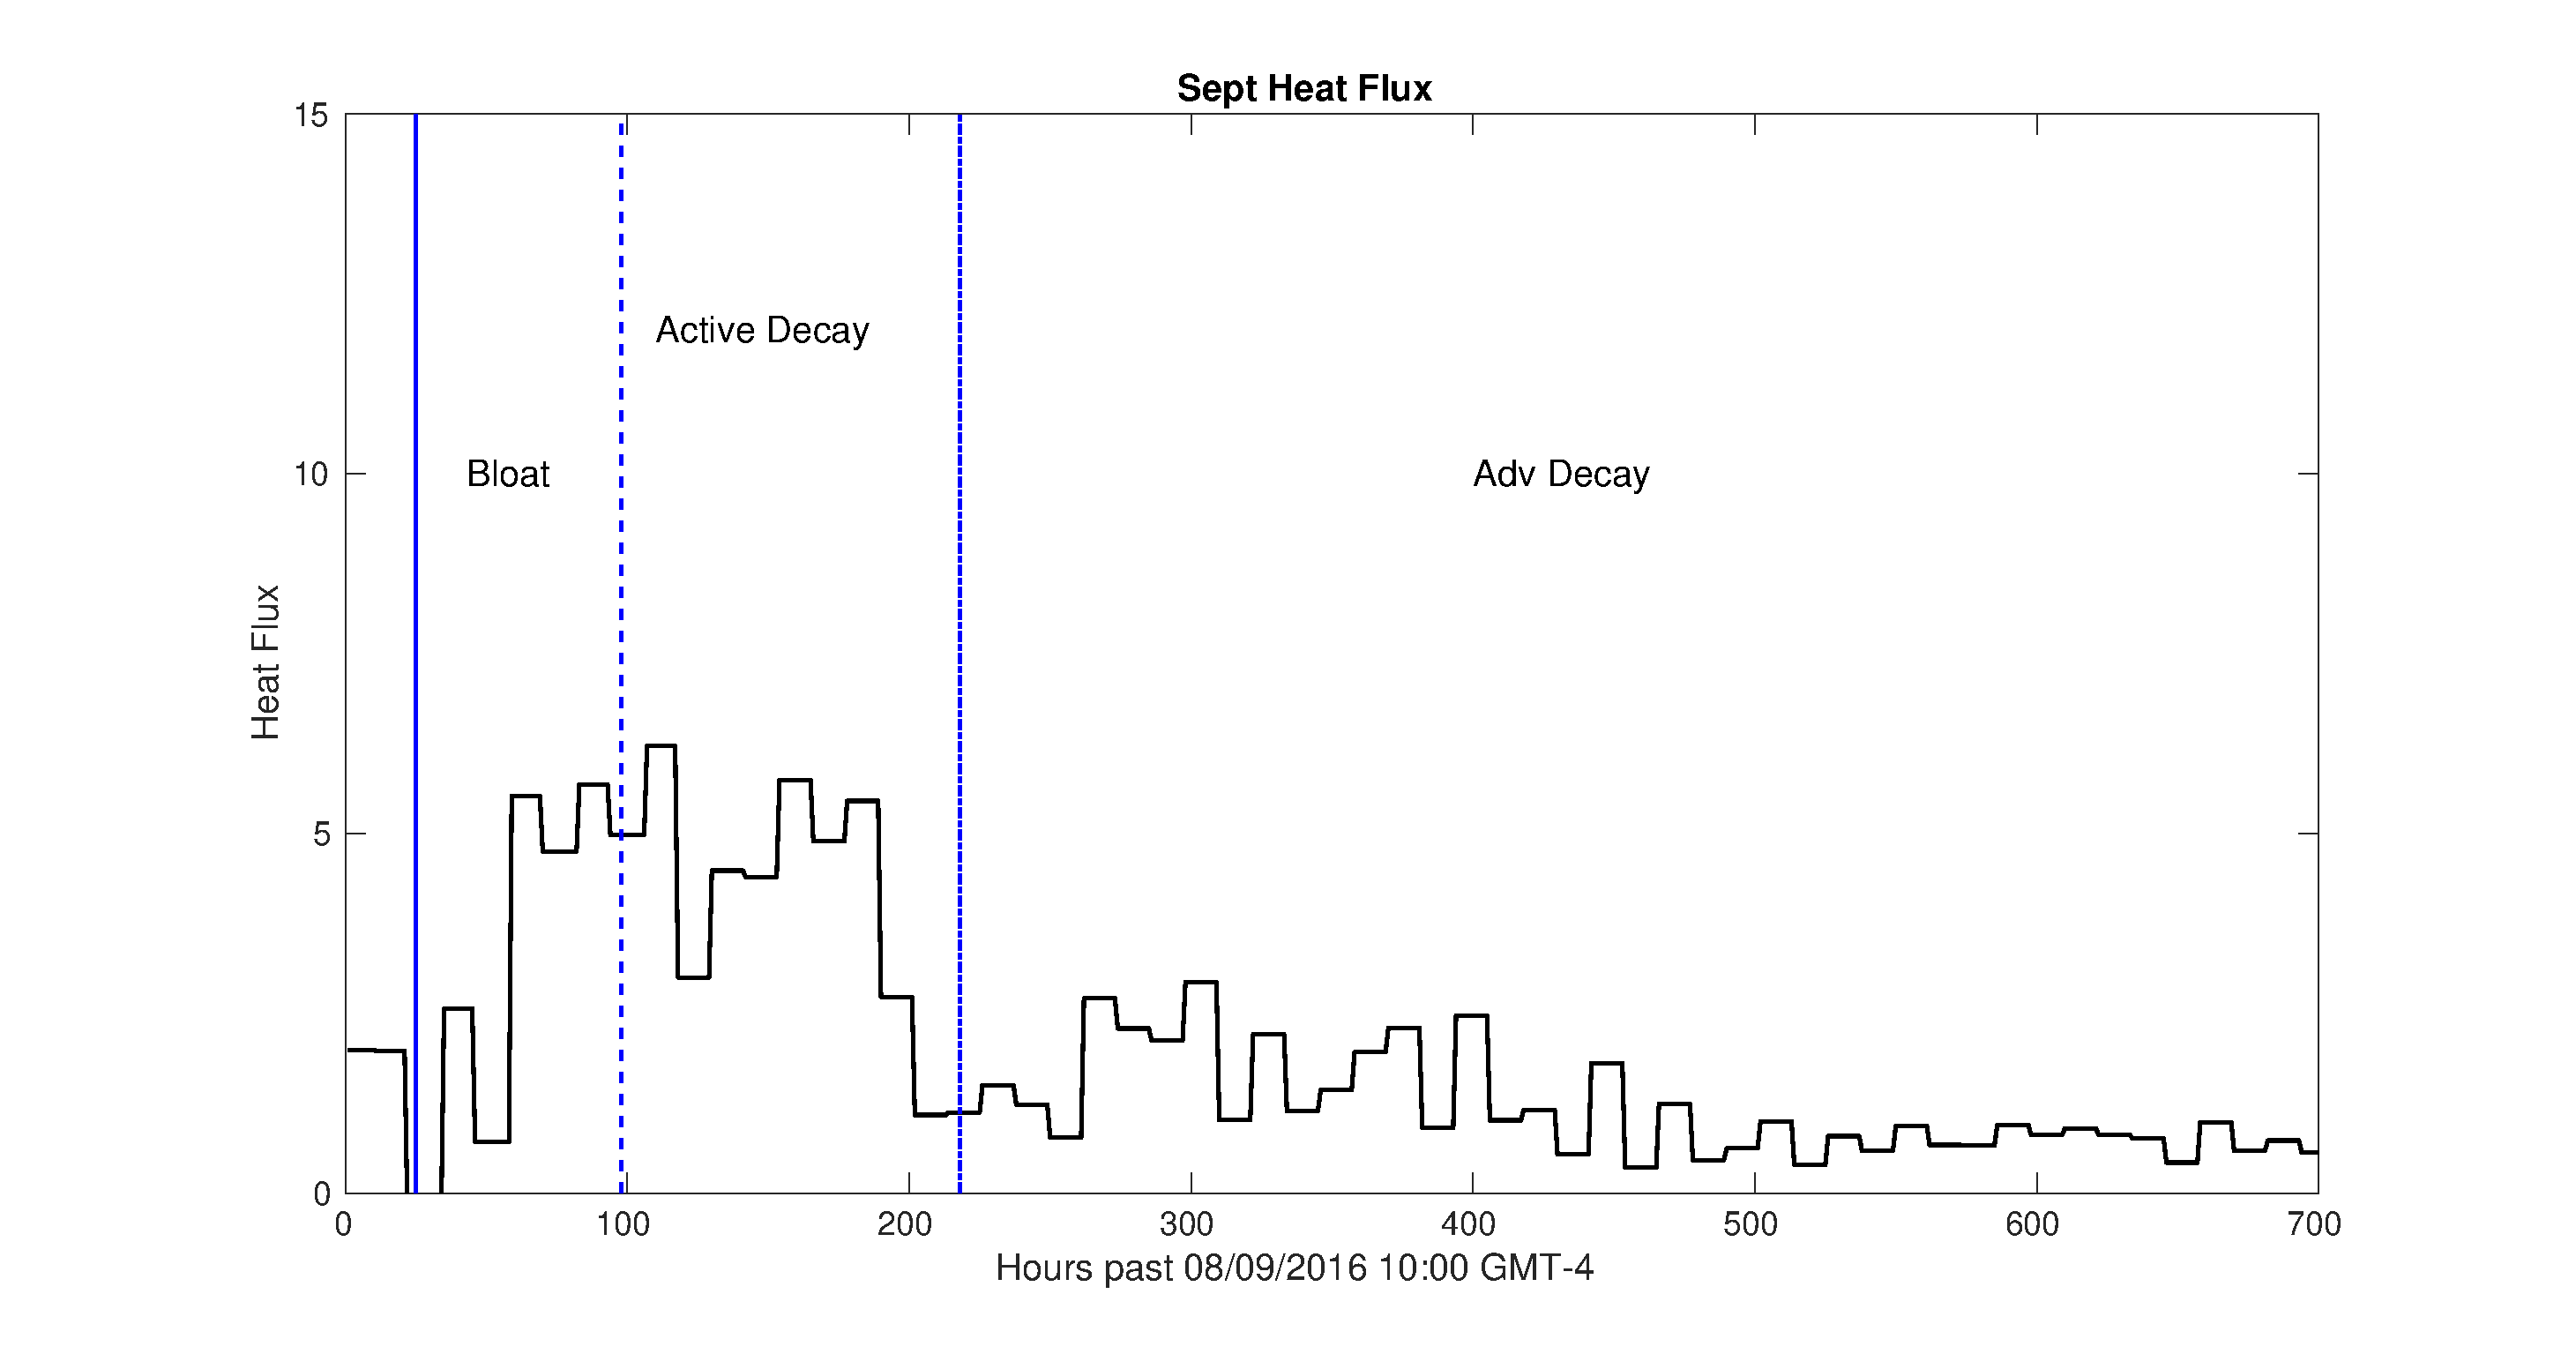
\includegraphics[width=0.49\textwidth]{Figures/sept_s_part}
  \caption{Left: July data set. Right:September data set. Hours past
    beginning of experiment plotted as the independent axis. Vertical
    lines indicate progression through observed stages of decomposition.}
\end{figure}
\end{frame}

\begin{frame}
  We also examine the heat flux signature as it depends on the ADD.
  \begin{figure}
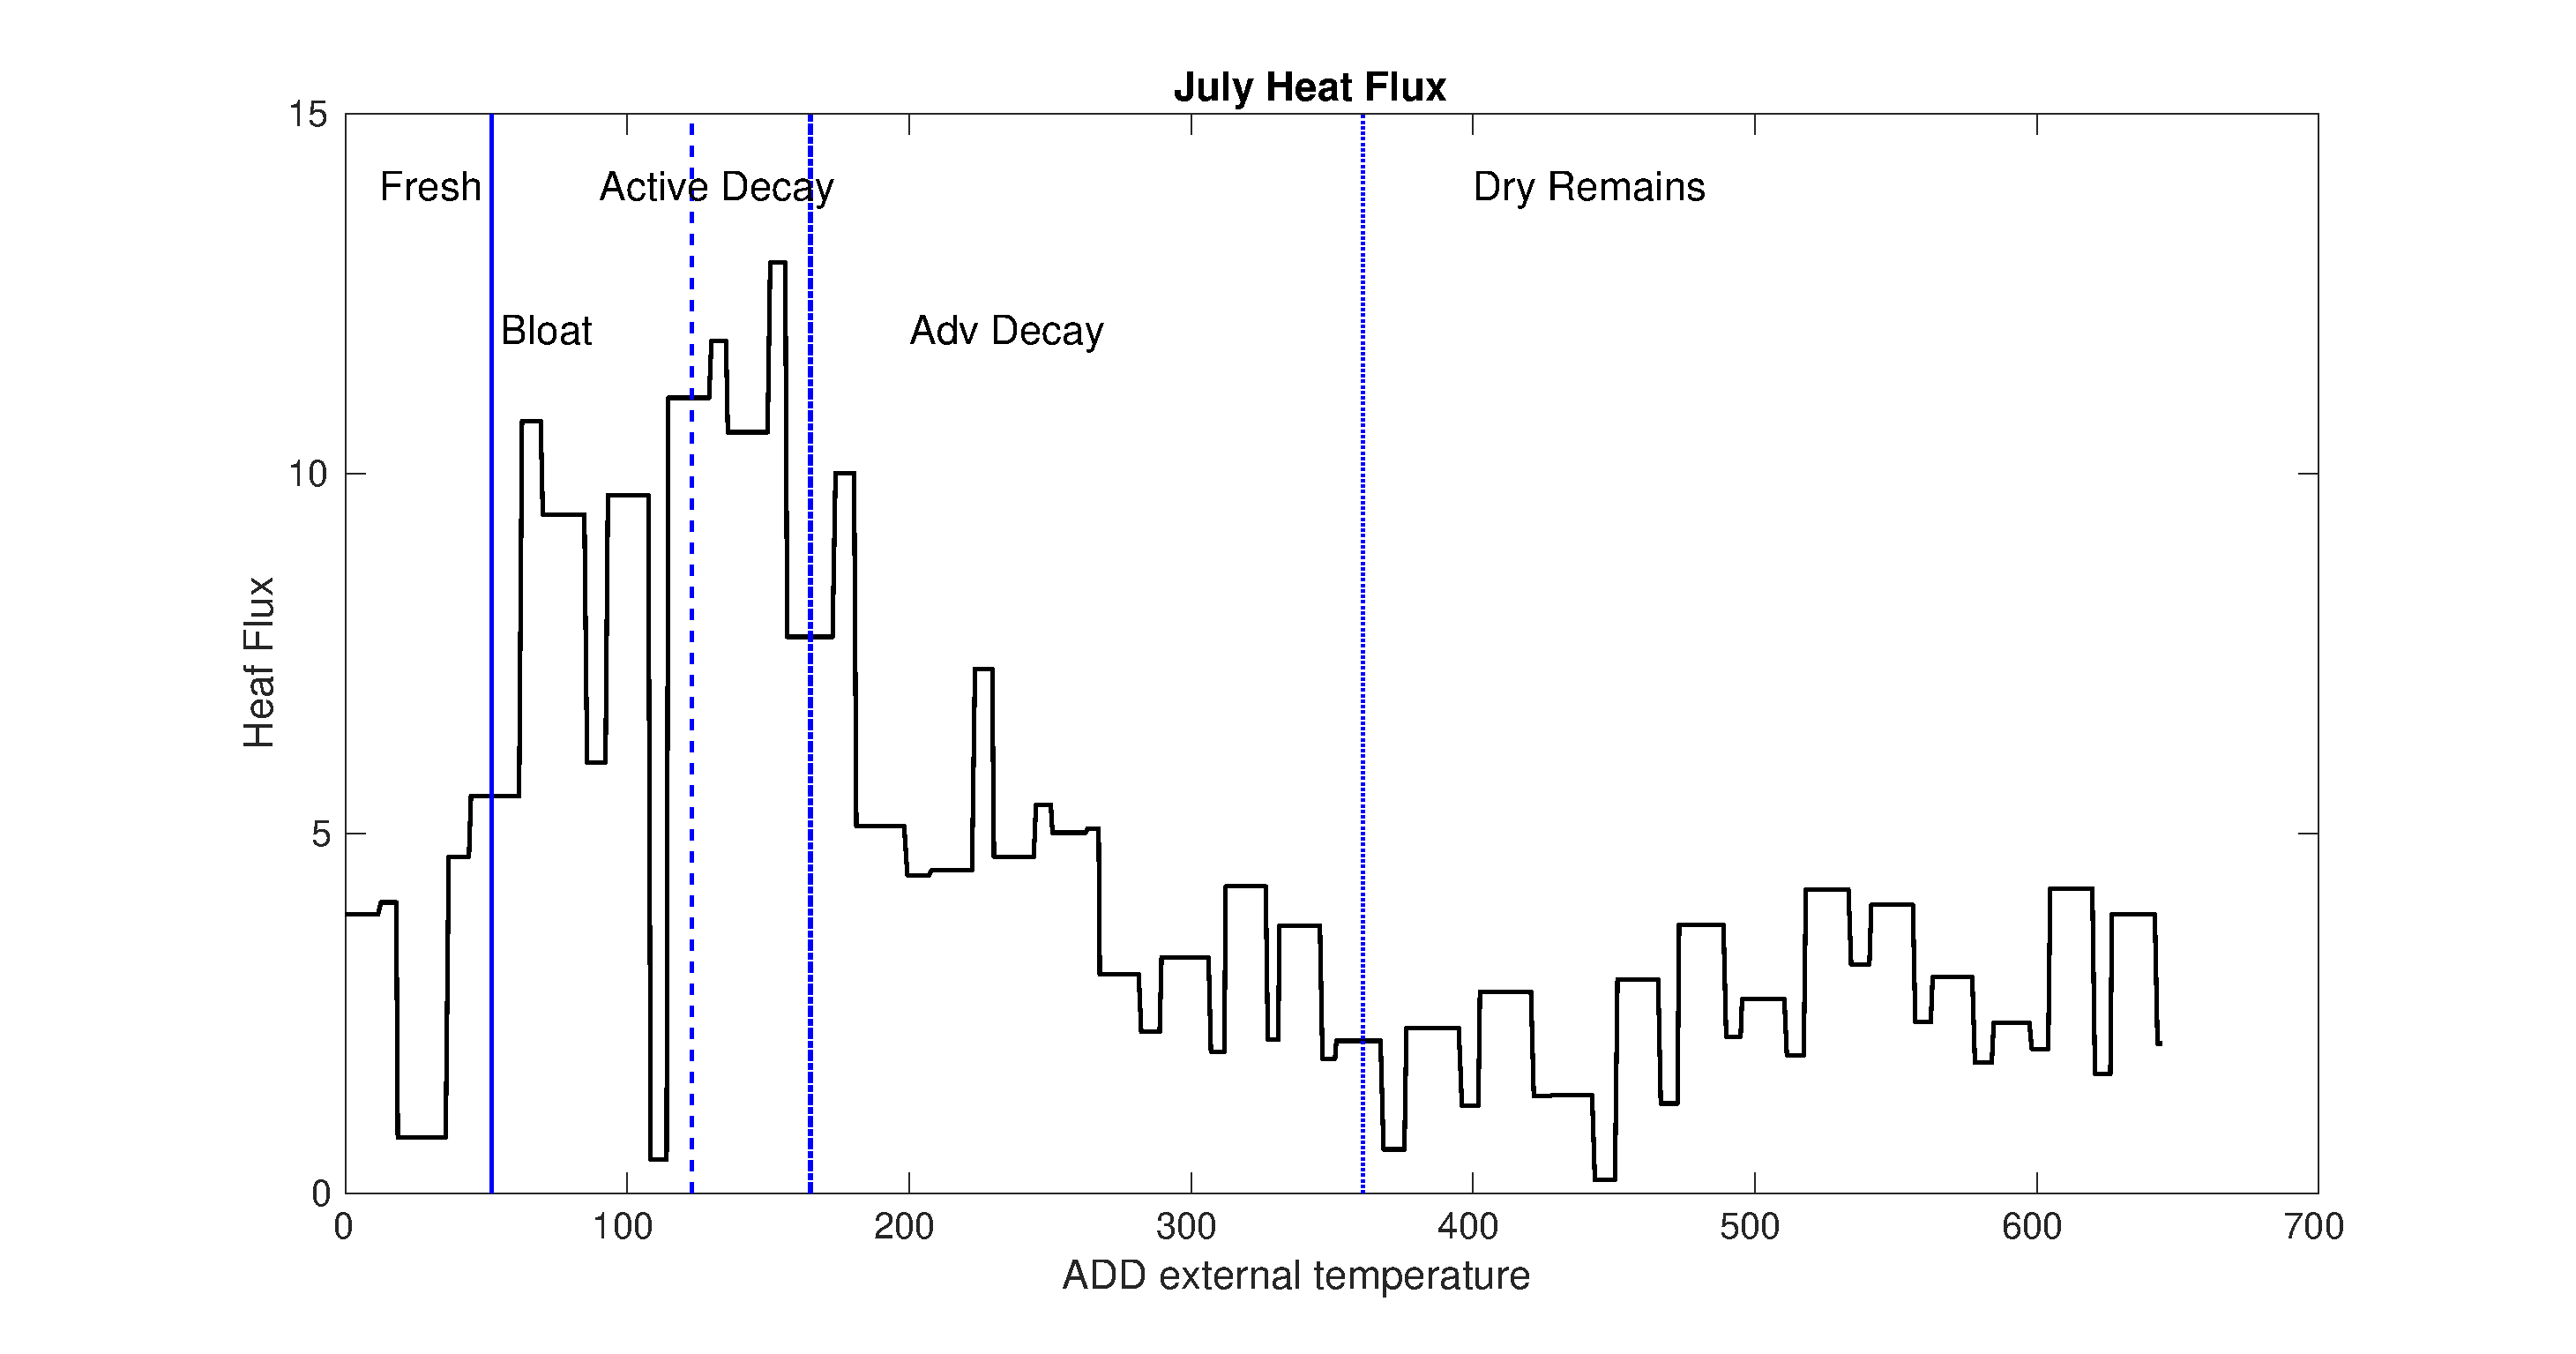
\includegraphics[width=0.49\textwidth]{Figures/jul_addex}
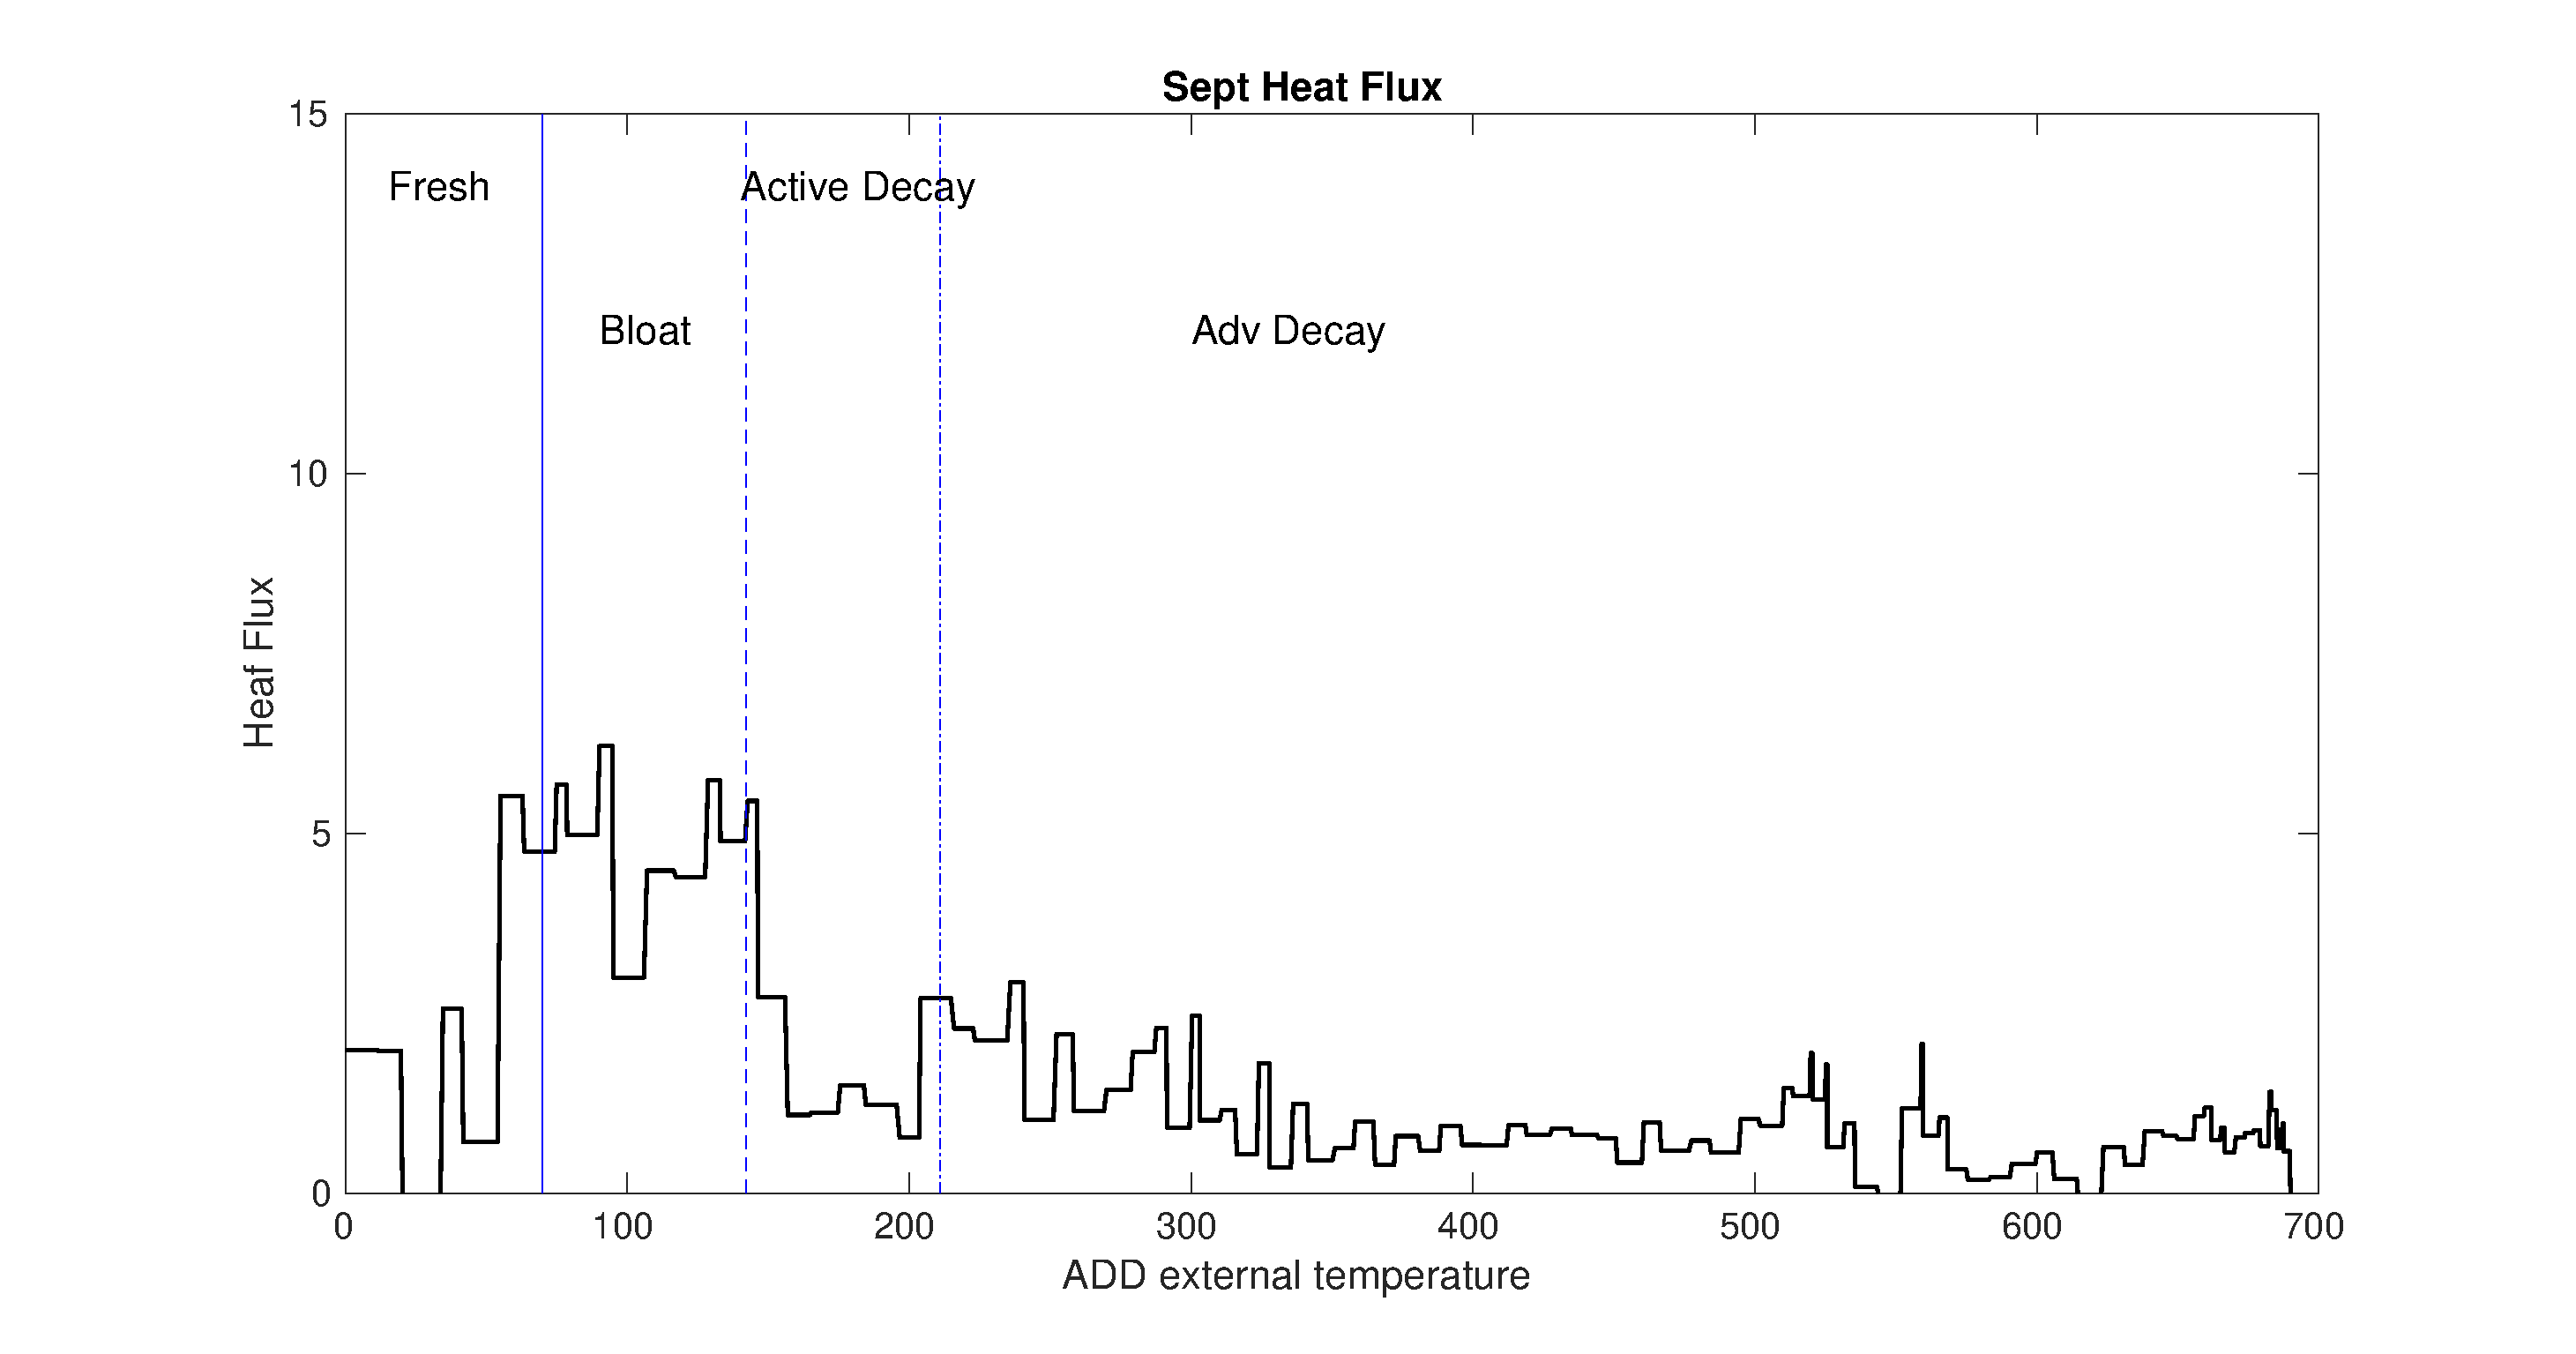
\includegraphics[width=0.49\textwidth]{Figures/sept_addex}
\caption{A scaling of the flux $\mathbf{s}^*$ with the 
abscissa expressed in ADD calculated using the external 
ambient temperature.}
\label{fig:s-fun-ADD}
\end{figure}
\end{frame}

\section{Temperature Prediction}


\end{document}
